% !TEX program = xelatex
\documentclass[12pt,a4paper]{article}

\usepackage{fontspec}
\usepackage{polyglossia}
\setmainlanguage{greek}
\setotherlanguage{english}
\setmainfont[Script=Greek]{DejaVu Serif}
\setsansfont[Script=Greek]{DejaVu Sans}
\setmonofont[Script=Greek]{DejaVu Sans Mono}
\newfontfamily\greekfonttt[Script=Greek]{DejaVu Sans Mono}

\usepackage[a4paper, margin=2.35cm]{geometry}
\usepackage{amsmath, amssymb}
\usepackage{booktabs}
\usepackage{array}
\usepackage{longtable}
\usepackage{graphicx}
\usepackage{float}
\usepackage{caption}
\usepackage[hidelinks]{hyperref}
\usepackage{enumitem}
\usepackage{parskip}
\usepackage{xcolor}
\usepackage{fancyhdr}
\usepackage{tcolorbox}
\tcbuselibrary{skins,breakable}

\pagestyle{fancy}
\fancyhf{}
\lhead{Τεχνικές και Οργάνωση Ελέγχου Ποιότητας}
\rhead{Explanatory Report V2}
\cfoot{\thepage}
\setlength{\headheight}{14.5pt}

\captionsetup{font=small, labelfont=bf}
\graphicspath{{./}}
\renewcommand{\arraystretch}{1.22}
\setlength{\parindent}{0pt}
\sloppy

\newcommand{\code}[1]{\texttt{\textenglish{#1}}}
\newcommand{\Pa}{P_{\!a}}
\newcommand{\AOQ}{\textenglish{AOQ}}
\newcommand{\AOQL}{\textenglish{AOQL}}
\newcommand{\ATI}{\textenglish{ATI}}
\newcommand{\ASN}{\textenglish{ASN}}
\newcommand{\AQL}{\textenglish{AQL}}
\newcommand{\OC}{\textenglish{OC}}
\newcommand{\ARL}{\textenglish{ARL}}

% --- Custom boxes for didactic callouts ----------------------------------
\newtcolorbox{intuition}[1][]{
    colback=blue!4!white, colframe=blue!55!black,
    boxrule=0.4pt, arc=2pt,
    title=\textbf{Διαίσθηση}, fonttitle=\bfseries,
    breakable, #1
}
\newtcolorbox{trap}[1][]{
    colback=red!4!white, colframe=red!55!black,
    boxrule=0.4pt, arc=2pt,
    title=\textbf{Παγίδα κατανόησης}, fonttitle=\bfseries,
    breakable, #1
}
\newtcolorbox{example}[1][]{
    colback=green!3!white, colframe=green!45!black,
    boxrule=0.4pt, arc=2pt,
    title=\textbf{Μικρό παράδειγμα}, fonttitle=\bfseries,
    breakable, #1
}
\newtcolorbox{summarybox}[1][]{
    colback=gray!8!white, colframe=gray!55!black,
    boxrule=0.4pt, arc=2pt,
    title=\textbf{Σύνοψη ερωτήματος}, fonttitle=\bfseries,
    breakable, #1
}

\title{
    \textbf{Τεχνικές και Οργάνωση Ελέγχου Ποιότητας}\\[0.25cm]
    \Large Αναλυτικό Explanatory Report (V2)\\[0.15cm]
    \large Δειγματοληπτικός έλεγχος αποδοχής και διαγράμματα ελέγχου,\\
    γραμμένο ως πλήρες εκπαιδευτικό κείμενο
}
\author{Τσακιρίδης}
\date{\today}

\begin{document}

\maketitle
\thispagestyle{fancy}

\begin{abstract}
Αυτό το report γράφτηκε από την αρχή για κάποιον που δεν έχει ξανασυναντήσει
τις έννοιες του στατιστικού ελέγχου ποιότητας. Πριν εμφανιστεί οποιαδήποτε
πράξη, εξηγείται με απλά λόγια τι θέλει να πετύχει η εργασία, ποια θεωρία
χρειάζεται και γιατί ο κάθε τύπος έχει τη μορφή που έχει. Στη συνέχεια οι
πράξεις γίνονται βήμα προς βήμα, με τις ενδιάμεσες τιμές να φαίνονται όλες,
ώστε ο αναγνώστης να μπορεί να αναπαράγει μόνος του τα αποτελέσματα. Η
εργασία αποτελείται από δύο μέρη: στο Μέρος Α σχεδιάζεται δειγματοληπτικός
έλεγχος αποδοχής παρτίδων με διαλογή και στο Μέρος Β κατασκευάζονται
διαγράμματα ελέγχου της μέσης τιμής και της τυπικής απόκλισης για την τάση
εξόδου ηλεκτρονικών τροφοδοτικών.
\end{abstract}

\tableofcontents
\newpage

%=============================================================================
\section*{Πώς να διαβαστεί αυτό το report}
\addcontentsline{toc}{section}{Πώς να διαβαστεί αυτό το report}
%=============================================================================

Το κείμενο είναι οργανωμένο έτσι ώστε να μπορεί να διαβαστεί γραμμικά, από
την αρχή έως το τέλος, χωρίς να χρειάζεται κανένα προηγούμενο μάθημα. Κάθε
ερώτημα της εργασίας ακολουθεί την ίδια τριμερή δομή:

\begin{enumerate}[leftmargin=2.2em]
    \item \textbf{Τι ζητάει το ερώτημα.} Η εκφώνηση ξαναγράφεται με απλά λόγια,
    χωρίς ορολογία, ώστε να ξέρουμε τι ψάχνουμε.
    \item \textbf{Θεωρητικό υπόβαθρο.} Παρουσιάζονται οι έννοιες και οι τύποι
    που χρειάζονται, με αναφορά στις γενικές ενότητες θεωρίας του κειμένου,
    και με σύντομα παραδείγματα διαίσθησης.
    \item \textbf{Λύση βήμα προς βήμα.} Παίρνουμε τις παραμέτρους, βάζουμε στους
    τύπους τους αριθμούς, εμφανίζουμε όλους τους ενδιάμεσους υπολογισμούς και
    βγάζουμε το τελικό αποτέλεσμα.
\end{enumerate}

Επιπλέον, υπάρχουν τρία είδη πλαισίων που εμφανίζονται μέσα στο κείμενο για
να βοηθήσουν την κατανόηση:

\begin{itemize}[leftmargin=2.2em]
    \item Τα μπλε πλαίσια \emph{Διαίσθηση} εξηγούν με αναλογίες ή απλά λόγια
    γιατί ένας τύπος έχει συγκεκριμένη μορφή.
    \item Τα κόκκινα πλαίσια \emph{Παγίδα κατανόησης} σηματοδοτούν συνηθισμένες
    παρανοήσεις και τις διορθώνουν.
    \item Τα πράσινα πλαίσια \emph{Μικρό παράδειγμα} δίνουν μια αριθμητική
    εικόνα με μικρές τιμές, ώστε ο τύπος να γίνει χειροπιαστός.
\end{itemize}

Οι αριθμοί όλου του report προέρχονται από το αρχείο \code{toep\_solution.py},
που λύνει την εργασία σε Python χρησιμοποιώντας τις βιβλιοθήκες \code{numpy},
\code{pandas} και \code{scipy}. Τα γραφήματα και τα ενδιάμεσα CSV βρίσκονται
στον ίδιο φάκελο με το παρόν κείμενο.

\newpage

%=============================================================================
\section*{Γλωσσάρι και πίνακας συμβόλων}
\addcontentsline{toc}{section}{Γλωσσάρι και πίνακας συμβόλων}
%=============================================================================

Πριν ξεκινήσουμε, παραθέτουμε σε έναν πίνακα όλα τα σύμβολα και τους όρους
που θα χρησιμοποιηθούν. Ο πίνακας είναι σχεδιασμένος ώστε να μπορεί να
ξανακοιτάζεται οποτεδήποτε. Αν κάποιο σύμβολο δεν είναι αμέσως κατανοητό,
αρκεί να επιστρέψετε εδώ.

\begin{longtable}{>{\centering\arraybackslash}p{2.0cm} p{12.2cm}}
\toprule
\textbf{Σύμβολο} & \textbf{Τι σημαίνει} \\
\midrule
\endfirsthead
\toprule
\textbf{Σύμβολο} & \textbf{Τι σημαίνει} \\
\midrule
\endhead
\(N\) & Μέγεθος παρτίδας. Πόσα εξαρτήματα έχει κάθε παρτίδα που παραλαμβάνουμε. \\
\(n\) & Μέγεθος δείγματος. Πόσα εξαρτήματα ελέγχουμε από την παρτίδα. \\
\(c\) & Αριθμός αποδοχής. Το πολύ τόσα ελαττωματικά επιτρέπονται στο δείγμα για να γίνει η παρτίδα αποδεκτή. \\
\(p\) & Πραγματικό ποσοστό ελαττωματικών μέσα σε μια παρτίδα. \\
\(p_1\) & Αποδεκτή στάθμη ποιότητας (ΑΣΠ). Το \(p\) μιας ``καλής'' παρτίδας. \\
\(p_2\) & Κακή στάθμη ποιότητας. Στην εργασία \(p_2=7p_1\). \\
\(\alpha\) & Κίνδυνος παραγωγού. Πιθανότητα να απορρίψουμε μια καλή παρτίδα. \\
\(\beta\) & Κίνδυνος πελάτη. Πιθανότητα να αποδεχτούμε μια κακή παρτίδα. \\
\(\Pa(p)\) & Πιθανότητα να γίνει αποδεκτή μια παρτίδα με ποσοστό ελαττωματικών \(p\). \\
\(\OC\) & Operating Characteristic. Η γραφική παράσταση του \(\Pa(p)\) ως προς \(p\). \\
\(\AOQ(p)\) & Μέση εξερχόμενη ποιότητα. Πόσα ελαττωματικά κατά μέσο όρο διαφεύγουν από το σχήμα. \\
\(\AOQL\) & Το μέγιστο της \(\AOQ(p)\) ως προς \(p\). Η χειρότερη μέση εξερχόμενη ποιότητα που μπορεί να συμβεί. \\
\(\ATI(p)\) & Μέσος συνολικός αριθμός εξαρτημάτων που ελέγχονται ανά παρτίδα. \\
\(\ASN(p)\) & Μέσος αριθμός δειγματικών μονάδων σε διπλό σχήμα. \\
\(c_i\) & Κόστος ελέγχου ενός εξαρτήματος. \\
\(c_d\) & Κόστος ενός ελαττωματικού που διαφεύγει και φτάνει στον πελάτη. \\
\(\mu_0\) & Στόχος της μέσης τιμής μιας παραγωγικής διαδικασίας. \\
\(\sigma\) & Τυπική απόκλιση των μετρήσεων όταν η διαδικασία είναι κανονική. \\
\(\bar X\) & Δειγματική μέση τιμή (αριθμητικός μέσος όρος ενός δείγματος). \\
\(S\) & Δειγματική τυπική απόκλιση. \\
\(LCL\), \(CL\), \(UCL\) & Κάτω, κεντρικό και άνω όριο ενός διαγράμματος ελέγχου. \\
\(k\) & Πόσες τυπικές αποκλίσεις απέχουν τα όρια ελέγχου από το κεντρικό όριο. \\
\(c_4\) & Συντελεστής διόρθωσης ώστε \(c_4\sigma\) να ισούται με τη μέση τιμή του \(S\). \\
\(\Delta\) & Πιθανή μετατόπιση της μέσης τιμής της διαδικασίας. \\
\(\ARL\) & Average Run Length. Μέσος αριθμός δειγμάτων μέχρι το διάγραμμα να δώσει ένδειξη. \\
\bottomrule
\end{longtable}

Οι όροι παραγωγός, πελάτης και διαλογή θα εξηγηθούν αναλυτικά στις
αντίστοιχες ενότητες, αλλά αξίζει εδώ μια πρώτη επαφή.

\textbf{Παραγωγός} είναι η πλευρά που φτιάχνει τις παρτίδες. \textbf{Πελάτης}
είναι η πλευρά που τις παραλαμβάνει. \textbf{Διαλογή} σημαίνει ότι όταν μια
παρτίδα απορρίπτεται από το δειγματοληπτικό σχήμα, ελέγχεται μετά 100\%, και
τα ελαττωματικά που βρίσκονται αφαιρούνται ή επισκευάζονται.

\newpage

%=============================================================================
\section{Αρχικά δεδομένα και πρώτη εικόνα του προβλήματος}
%=============================================================================

\subsection{Γιατί χρειάζεται έλεγχος ποιότητας}

Σε κάθε βιομηχανική παραγωγή, καμία διαδικασία δεν παράγει αποκλειστικά τέλεια
προϊόντα. Πάντα υπάρχει κάποιο ποσοστό ελαττωματικών, λόγω φθοράς μηχανών,
θερμοκρασιακών μεταβολών, ανθρώπινου παράγοντα, διαφορών στη πρώτη ύλη και
ασήμαντων διακυμάνσεων που είναι αδύνατο να αποφευχθούν.

Δύο είναι τα ερωτήματα που μας απασχολούν συνεχώς:

\begin{enumerate}[leftmargin=2.2em]
    \item Παραλαμβάνω μια παρτίδα. Είναι αρκετά καλή για να τη δεχτώ;
    \item Λειτουργώ μια γραμμή παραγωγής. Συμπεριφέρεται σήμερα όπως
    συμπεριφερόταν χθες, ή κάτι έχει αλλάξει;
\end{enumerate}

Το πρώτο ερώτημα αντιμετωπίζεται με \emph{δειγματοληπτικό έλεγχο αποδοχής},
που είναι το αντικείμενο του Μέρους Α. Το δεύτερο αντιμετωπίζεται με
\emph{διαγράμματα ελέγχου διαδικασίας}, που είναι το αντικείμενο του
Μέρους Β.

\begin{intuition}
Σκεφτείτε ότι παραλαμβάνετε ένα φορτίο με χιλιάδες μήλα. Δεν μπορείτε να τα
ελέγξετε όλα ένα προς ένα. Παίρνετε ένα τυχαίο σακούλι και κοιτάτε αν έχει
χτυπημένα μήλα. Με βάση αυτό το μικρό δείγμα αποφασίζετε για ολόκληρο το
φορτίο. Αυτή είναι ακριβώς η ιδέα του δειγματοληπτικού ελέγχου αποδοχής.
\end{intuition}

\subsection{Παράμετροι του Μέρους Α}

Στο Μέρος Α παραλαμβάνουμε παρτίδες των \(N=600\) εξαρτημάτων. Κάθε
παράμετρος που εμφανίζεται στην εκφώνηση έχει τη δική της φυσική σημασία.

\begin{table}[H]
\centering
\caption{Δεδομένα Μέρους Α και τι αντιπροσωπεύει το καθένα.}
\small
\begin{tabular}{>{\centering\arraybackslash}p{1.8cm}>{\centering\arraybackslash}p{1.8cm}p{9.7cm}}
\toprule
\textbf{Σύμβολο} & \textbf{Τιμή} & \textbf{Ερμηνεία} \\
\midrule
\(N\) & 600 & Πλήθος εξαρτημάτων ανά παρτίδα. \\
\(c_i\) & 6 € & Κόστος ελέγχου ενός εξαρτήματος. \\
\(c_d\) & 400 € & Κόστος που υφίσταται η εταιρία αν ένα ελαττωματικό περάσει στον πελάτη. \\
\(p_1\) & 0,0065 & Αποδεκτή στάθμη ποιότητας (ΑΣΠ = 0,65\%). \\
\(\alpha\) & 0,03 & Μέγιστος επιτρεπτός κίνδυνος παραγωγού. \\
\(\beta\) & 0,10 & Μέγιστος επιτρεπτός κίνδυνος πελάτη. \\
\(p_2=7p_1\) & 0,0455 & Κακή στάθμη ποιότητας. \\
\(p_L\) & 0,004 & Κάτω άκρο τυχαίας κατανομής του \(p\) στο Ερώτημα Α4. \\
\(p_U\) & 0,060 & Άνω άκρο τυχαίας κατανομής του \(p\) στο Ερώτημα Α4. \\
\bottomrule
\end{tabular}
\end{table}

Δύο παρατηρήσεις είναι κρίσιμες:

\begin{itemize}[leftmargin=2.2em]
    \item Το \(c_d\) είναι περίπου \(67\) φορές μεγαλύτερο από το \(c_i\).
    Δηλαδή κάθε ελαττωματικό που διαφεύγει στοιχίζει πολύ περισσότερο από έναν
    απλό έλεγχο. Αυτό είναι ένα πολύ συνηθισμένο μοτίβο στη βιομηχανία και θα
    δικαιολογήσει αργότερα γιατί ο έλεγχος έχει νόημα.
    \item Το \(p_2\) δεν είναι αυθαίρετο. Η εργασία το ορίζει ως
    \(p_2=7p_1\). Είναι το ποσοστό ελαττωματικών που θεωρούμε αρκετά κακό
    ώστε να θέλουμε να το απορρίπτουμε με μεγάλη πιθανότητα.
\end{itemize}

\subsection{Παράμετροι του Μέρους Β}

Στο Μέρος Β το προϊόν είναι ηλεκτρονικό τροφοδοτικό και ελέγχουμε τη τάση
εξόδου. Η τάση πρέπει να βρίσκεται όσο γίνεται πιο κοντά στα 9 V.

\begin{table}[H]
\centering
\caption{Δεδομένα Μέρους Β.}
\small
\begin{tabular}{>{\centering\arraybackslash}p{1.8cm}>{\centering\arraybackslash}p{1.8cm}p{9.7cm}}
\toprule
\textbf{Σύμβολο} & \textbf{Τιμή} & \textbf{Ερμηνεία} \\
\midrule
\(\mu_0\) & 9 V & Στόχος μέσης τάσης εξόδου. \\
\(A\) & 0,10 V & Ημιπλάτος των ορίων προδιαγραφών. Δίνει το διάστημα 8,90--9,10 V. \\
\(\sigma\) & 0,035 V & Τυπική απόκλιση όταν η διαδικασία είναι εντός ελέγχου. \\
\(K\) & 21 € & Κόστος που πληρώνουμε για κάθε ελαττωματικό τροφοδοτικό που παράγουμε. \\
\(\Delta\) & 0,06 V & Πιθανή μεταβολή της μέσης τάσης. \\
\(k\) & 2,5 & Πόσες τυπικές αποκλίσεις απέχουν τα όρια ελέγχου από το κεντρικό όριο. \\
\(n\) & 5 & Μέγεθος δείγματος που παίρνουμε κάθε ώρα. \\
\bottomrule
\end{tabular}
\end{table}

Τα όρια προδιαγραφών είναι:
\[
    LSL = \mu_0 - A = 9 - 0{,}10 = 8{,}90 \text{ V},
\]
\[
    USL = \mu_0 + A = 9 + 0{,}10 = 9{,}10 \text{ V}.
\]

Ένα τροφοδοτικό θεωρείται αποδεκτό αν η τάση του βρίσκεται μέσα σε αυτό το
διάστημα.

\begin{trap}
Τα όρια προδιαγραφών (\(LSL\), \(USL\)) δεν είναι το ίδιο πράγμα με τα όρια
ελέγχου (\(LCL\), \(UCL\)). Τα όρια προδιαγραφών έρχονται από τις απαιτήσεις
του πελάτη ή του σχεδιαστή του προϊόντος. Τα όρια ελέγχου έρχονται από τη
στατιστική συμπεριφορά της \emph{δειγματικής} μέσης τιμής. Είναι δύο
διαφορετικά πράγματα και η σύγχυση είναι το πιο συχνό λάθος στις εργασίες
ποιοτικού ελέγχου.
\end{trap}

\newpage

%=============================================================================
\section{Στατιστικά θεμέλια του Μέρους Α}
%=============================================================================

Πριν λύσουμε οποιοδήποτε ερώτημα, ξεκαθαρίζουμε τη θεωρία στην οποία θα
στηριχτούμε. Όλο το Μέρος Α βασίζεται σε μία και μόνο κατανομή: τη
διωνυμική.

\subsection{Η διωνυμική κατανομή με απλά λόγια}

Φανταστείτε ότι έχουμε ένα κουτί με 600 μπίλιες. Ένα ποσοστό \(p\) από αυτές
είναι ελαττωματικές. Παίρνουμε ένα τυχαίο δείγμα \(n\) μπίλιων χωρίς να
ψάχνουμε επίτηδες. Πόσες θα είναι ελαττωματικές;

Δεν υπάρχει σταθερή απάντηση. Είναι τυχαίο πράγμα. Άλλη φορά μπορεί να βγουν
2 ελαττωματικές, άλλη φορά 5, άλλη φορά καμία.

Όταν το \(n\) είναι σχετικά μικρό σε σχέση με το \(N\), η πιθανότητα να βρούμε
ακριβώς \(x\) ελαττωματικά στο δείγμα δίνεται από τη διωνυμική κατανομή:
\[
    P(X=x)
    =
    \binom{n}{x}\,p^{x}\,(1-p)^{n-x}.
\]

Ας εξηγήσουμε κάθε όρο:

\begin{itemize}[leftmargin=2.2em]
    \item Το \(p^{x}\) είναι η πιθανότητα οι \(x\) συγκεκριμένες μπίλιες που
    διαλέγουμε να είναι όλες ελαττωματικές.
    \item Το \((1-p)^{n-x}\) είναι η πιθανότητα οι υπόλοιπες \(n-x\) μπίλιες
    να είναι όλες καλές.
    \item Το \(\binom{n}{x}\) μετράει με πόσους τρόπους μπορούν να επιλεγούν
    \(x\) ελαττωματικές μέσα σε δείγμα μεγέθους \(n\).
\end{itemize}

\begin{example}
Έστω \(n=10\) και \(p=0{,}1\). Πόση πιθανότητα έχουμε να βρούμε ακριβώς 2
ελαττωματικά;
\[
    P(X=2)=\binom{10}{2}(0{,}1)^2(0{,}9)^8
    =45\cdot 0{,}01\cdot 0{,}4305
    \approx 0{,}194.
\]
Δηλαδή περίπου 19,4\% πιθανότητα.
\end{example}

\subsection{Η αθροιστική διωνυμική}

Στις εφαρμογές δεν μας ενδιαφέρει συνήθως η πιθανότητα να βρούμε ακριβώς
\(x\) ελαττωματικά. Μας ενδιαφέρει η πιθανότητα να βρούμε το πολύ \(c\)
ελαττωματικά:
\[
    P(X\le c)=\sum_{x=0}^{c}\binom{n}{x}p^{x}(1-p)^{n-x}.
\]

Αυτή η συνάρτηση λέγεται \emph{αθροιστική διωνυμική} και είναι το κύριο
εργαλείο του Μέρους Α. Στον κώδικα Python εμφανίζεται ως:
\code{binom.cdf(c, n, p)}.

\subsection{Καμπύλη αποδοχής (OC)}

Όταν εφαρμόζουμε σχήμα \((n,c)\), η παρτίδα γίνεται αποδεκτή αν το δείγμα
έχει το πολύ \(c\) ελαττωματικά. Η πιθανότητα αποδοχής, ως συνάρτηση του
\(p\), είναι:
\[
    \Pa(p)=\sum_{x=0}^{c}\binom{n}{x}p^{x}(1-p)^{n-x}.
\]

Η γραφική παράσταση του \(\Pa(p)\) ως προς \(p\) λέγεται \emph{χαρακτηριστική
καμπύλη αποδοχής} ή \OC. Είναι το πιο σημαντικό εργαλείο για τη μελέτη ενός
σχήματος ελέγχου, γιατί συμπυκνώνει όλη του τη συμπεριφορά.

\begin{intuition}
Η \OC\ απαντάει στην ερώτηση: αν η πραγματικότητα ήταν τόσο κακή
(ποσοστό ελαττωματικών \(p\)), τι πιθανότητα έχει το σχήμα μου να αφήσει
την παρτίδα να περάσει; Όσο μεγαλώνει το \(p\), τόσο πρέπει να μικραίνει
η \(\Pa(p)\). Αν δεν μικραίνει αρκετά, το σχήμα είναι κακό.
\end{intuition}

\subsection{Κίνδυνοι παραγωγού και πελάτη}

Δύο σημεία της \OC\ είναι τα πιο σημαντικά:

\begin{itemize}[leftmargin=2.2em]
    \item Στο \(p_1\), το \(\Pa(p_1)\) πρέπει να είναι μεγάλο, ώστε να μην
    απορρίπτουμε τυχαία τις καλές παρτίδες.
    \item Στο \(p_2\), το \(\Pa(p_2)\) πρέπει να είναι μικρό, ώστε να μην
    αποδεχόμαστε τυχαία τις κακές παρτίδες.
\end{itemize}

Με σύμβολα:
\[
    \Pa(p_1)\ge 1-\alpha,\qquad \Pa(p_2)\le \beta.
\]

Στην εργασία \(\alpha=0{,}03\), δηλαδή το πολύ 3\% πιθανότητα να απορρίψουμε
καλή παρτίδα. Και \(\beta=0{,}10\), δηλαδή το πολύ 10\% πιθανότητα να
αποδεχτούμε κακή παρτίδα.

\begin{intuition}
Ο παραγωγός δείχνει ένα ευχαριστημένο πρόσωπο όταν μια καλή παρτίδα του
γίνεται αποδεκτή. Αν την απορρίψουμε ενώ ήταν καλή, χάνει χρόνο και χρήμα.
Ο πελάτης από την άλλη βλέπει με τρόμο να δέχεται μια κακή παρτίδα. Αυτό
έχει συνέπειες στους δικούς του πελάτες. Άρα τα \(\alpha\) και \(\beta\)
αντιστοιχούν στους δύο φόβους.
\end{intuition}

\subsection{Μέση εξερχόμενη ποιότητα (AOQ) και AOQL}

Είπαμε ότι έχουμε έλεγχο με διαλογή. Αυτό σημαίνει:

\begin{itemize}[leftmargin=2.2em]
    \item Όταν μια παρτίδα γίνει αποδεκτή, κρατάμε όλη την παρτίδα, αφού πρώτα
    έχουν αφαιρεθεί τα ελαττωματικά που βρέθηκαν στο δείγμα.
    \item Όταν μια παρτίδα απορριφθεί, την ελέγχουμε 100\%, αφαιρούμε όλα τα
    ελαττωματικά και την παραδίδουμε καθαρή.
\end{itemize}

Άρα τα μόνα ελαττωματικά που μπορούν να καταλήξουν στον πελάτη είναι αυτά που
βρίσκονται στις παρτίδες οι οποίες έγιναν αποδεκτές, και μάλιστα μόνο σε
αυτά τα εξαρτήματα που \emph{δεν} ήταν στο δείγμα.

Αν είναι \(p\) το αρχικό ποσοστό ελαττωματικών, τότε ο μέσος αριθμός
ελαττωματικών που διαφεύγουν ανά παρτίδα είναι:
\[
    p\,\Pa(p)\,(N-n).
\]

Διαιρώντας με το \(N\) παίρνουμε το ποσοστό ελαττωματικών που τελικά παίρνει
ο πελάτης, που λέγεται \emph{μέση εξερχόμενη ποιότητα}:
\[
    \AOQ(p)=p\,\Pa(p)\,\frac{N-n}{N}.
\]

\begin{intuition}
Διαβάστε τον τύπο όπως μια ιστορία.

\(p\): αρχικό ποσοστό προβληματικών.

\(\Pa(p)\): η παρτίδα πέρασε.

\(\frac{N-n}{N}\): μόνο όσα εξαρτήματα δεν ελέγχθηκαν μπορούν να ξεγλιστρήσουν.
\end{intuition}

Παρατηρούμε ότι το \(\AOQ(p)\) είναι 0 στα δύο άκρα. Όταν \(p=0\) η παρτίδα
είναι τέλεια. Όταν \(p\) μεγαλώνει, το \(\Pa(p)\) τείνει στο 0, οπότε η
παρτίδα δεν περνάει και πάλι δεν διαφεύγουν ελαττωματικά. Άρα κάπου στη μέση
υπάρχει ένα μέγιστο. Αυτό το μέγιστο λέγεται \emph{AOQL}.
\[
    \AOQL = \max_{p\in[0,1]}\AOQ(p).
\]

Το \(\AOQL\) δείχνει το χειρότερο σενάριο: όσο μη ευνοϊκή κι αν είναι η
πραγματικότητα ως προς το \(p\), η μέση εξερχόμενη ποιότητα δεν θα ξεπεράσει
την τιμή \(\AOQL\).

\subsection{Μέσος συνολικός αριθμός ελεγχόμενων μονάδων (ATI)}

Στο απλό σχήμα ελέγχουμε πάντα \(n\) μονάδες. Αν όμως απορριφθεί η παρτίδα,
ελέγχουμε επιπλέον τις \(N-n\) μονάδες που μένουν. Άρα ο μέσος συνολικός
αριθμός είναι:
\[
    \ATI(p)=n+(N-n)\bigl[1-\Pa(p)\bigr].
\]

Όταν \(\Pa(p)\) είναι κοντά στο 1, η \(\ATI(p)\) είναι κοντά στο \(n\).
Όταν \(\Pa(p)\) είναι κοντά στο 0, η \(\ATI(p)\) είναι κοντά στο \(N\).

\newpage

%=============================================================================
\section{Μέρος Α: Δειγματοληπτικός έλεγχος αποδοχής}
%=============================================================================

\subsection{Γενική εικόνα του Μέρους Α}

Η εταιρία παραλαμβάνει συνέχεια παρτίδες των 600 εξαρτημάτων από έναν
προμηθευτή. Δεν θέλει ούτε να ελέγχει πάντα τα 600, ούτε να μη κάνει κανέναν
έλεγχο. Δοκιμάζει λοιπόν δειγματοληπτικά σχήματα, που είναι μια συμβιβαστική
λύση.

\begin{intuition}
Φανταστείτε ότι είστε γεωπόνος και παραλαμβάνετε μια μπάλα από κιβώτια με
ροδάκινα. Αν ανοίξετε όλα τα κιβώτια, χάνετε όλη τη μέρα. Αν δεν ανοίξετε
κανένα, μπορεί να βάλετε σάπια ροδάκινα στο σούπερ μάρκετ. Ανοίγετε λοιπόν
μερικά κιβώτια και μετράτε. Αν τα σάπια είναι πολλά, ανοίγετε όλη την
παραλαβή. Αυτή είναι ακριβώς η ιδέα του σχήματος αποδοχής με διαλογή.
\end{intuition}

%-----------------------------------------------------------------------------
\subsection{Ερώτημα Α1: Απλό δειγματοληπτικό σχήμα}
%-----------------------------------------------------------------------------

\subsubsection*{Τι ζητάει το ερώτημα}

Ζητείται απλό σχήμα ελέγχου της μορφής \((n,c)\). Η εκφώνηση επιβάλλει τρεις
ταυτόχρονες απαιτήσεις:

\begin{enumerate}[leftmargin=2.2em]
    \item Ο κίνδυνος του παραγωγού στο \(p_1\) να μην υπερβαίνει το \(\alpha\):
    \[
        1-\Pa(p_1)\le \alpha.
    \]
    \item Ο κίνδυνος του πελάτη στο \(p_2=7p_1\) να μην υπερβαίνει το \(\beta\):
    \[
        \Pa(p_2)\le \beta.
    \]
    \item Το \(\AOQL\) του σχήματος να μην υπερβαίνει το \(3p_1\):
    \[
        \AOQL\le 3p_1.
    \]
\end{enumerate}

\begin{summarybox}
Δοθέντος ότι \(p_1=0{,}0065\), έχουμε \(p_2=0{,}0455\) και \(3p_1=0{,}0195\).
Άρα ψάχνουμε ζεύγος \((n,c)\) τέτοιο ώστε:
\[
    \Pa(0{,}0065)\ge 0{,}97,\quad \Pa(0{,}0455)\le 0{,}10,\quad \AOQL\le 0{,}0195.
\]
\end{summarybox}

\subsubsection*{Πώς ψάχνουμε τη λύση}

Δεν υπάρχει αναλυτικός τύπος που να μας δίνει κατευθείαν το ζεύγος \((n,c)\).
Στην πράξη δοκιμάζουμε. Ο αλγόριθμος είναι:

\begin{enumerate}[leftmargin=2.2em]
    \item Ξεκινάμε από \(n=1\) και αυξάνουμε σταδιακά.
    \item Για κάθε \(n\), δοκιμάζουμε \(c=0,1,2,\dots\)
    \item Για κάθε ζεύγος \((n,c)\) υπολογίζουμε \(\Pa(p_1)\), \(\Pa(p_2)\)
    και \(\AOQL\).
    \item Αν ικανοποιούνται και οι τρεις περιορισμοί, καταγράφουμε το ζεύγος.
    \item Επιλέγουμε το ζεύγος με το μικρότερο \(n\) ως πιο οικονομικό σε
    ελέγχους.
\end{enumerate}

Αυτή ακριβώς η λογική υλοποιείται στη συνάρτηση
\code{find\_single\_plan} του \code{toep\_solution.py}.

\subsubsection*{Αποτέλεσμα και ερμηνεία}

Το πρώτο εφικτό ζεύγος που εντοπίζεται είναι:
\[
    \boxed{n=145,\qquad c=3}.
\]

Πρακτικά αυτό σημαίνει:

\begin{itemize}[leftmargin=2.2em]
    \item Από κάθε παρτίδα των 600 παίρνουμε τυχαίο δείγμα 145 εξαρτημάτων.
    \item Μετράμε πόσα είναι ελαττωματικά μέσα στο δείγμα.
    \item Αν τα ελαττωματικά είναι 0, 1, 2 ή 3, αποδεχόμαστε την παρτίδα.
    \item Αν είναι 4 ή περισσότερα, απορρίπτουμε την παρτίδα και την ελέγχουμε
    όλη (100\%).
\end{itemize}

\begin{table}[H]
\centering
\caption{Χαρακτηριστικά μεγέθη του απλού σχήματος του Α1.}
\begin{tabular}{lr}
\toprule
\textbf{Μέγεθος} & \textbf{Τιμή} \\
\midrule
\(n\) & 145 \\
\(c\) & 3 \\
\(\Pa(p_1)\) & 0,98470 \\
\(1-\Pa(p_1)\) (κίνδυνος παραγωγού) & 0,01530 \\
\(\Pa(p_2)\) (κίνδυνος πελάτη) & 0,09993 \\
\(\AOQL\) & 0,01016 \\
\(p\) όπου εμφανίζεται το \(\AOQL\) & 0,02021 \\
\(\ATI(p_1)\) & 151,96 \\
\(\ATI(p_2)\) & 554,53 \\
\bottomrule
\end{tabular}
\end{table}

Ελέγχουμε ότι όντως ικανοποιούνται όλες οι απαιτήσεις της εκφώνησης:

\textbf{Κίνδυνος παραγωγού.}
\[
    1-\Pa(p_1)=1-0{,}98470=0{,}01530.
\]
Σύγκριση: \(0{,}01530 < 0{,}03\). \checkmark

\textbf{Κίνδυνος πελάτη.}
\[
    \Pa(p_2)=0{,}09993.
\]
Σύγκριση: \(0{,}09993 < 0{,}10\). \checkmark

\textbf{AOQL.}
\[
    \AOQL=0{,}01016.
\]
Σύγκριση: \(0{,}01016 < 0{,}0195\). \checkmark

\begin{intuition}
Παρατηρήστε το \(\ATI(p_1)=151{,}96\). Αυτό σημαίνει ότι όταν οι παρτίδες
είναι καλές, ελέγχουμε κατά μέσο όρο 152 από τις 600 μονάδες. Αντίθετα,
όταν οι παρτίδες είναι κακές, \(\ATI(p_2)=554{,}53\). Σχεδόν ολόκληρη η
παρτίδα ελέγχεται. Αυτή ακριβώς είναι η ιδέα της διαλογής: η κακή ποιότητα
τιμωρείται με 100\% έλεγχο.
\end{intuition}

\begin{trap}
Κάποιοι σκέφτονται: ``αν \(c=3\), αυτό σημαίνει ότι δέχομαι το πολύ 3
ελαττωματικά στην παρτίδα''. \textbf{Αυτό είναι λάθος.} Το \(c=3\) αφορά
\emph{το δείγμα}, όχι την παρτίδα. Στην παρτίδα μπορεί να έχει συνολικά
πολύ περισσότερα ελαττωματικά. Στο δείγμα μόνο επιτρέπουμε έως 3 για να
γίνει αποδοχή.
\end{trap}

%-----------------------------------------------------------------------------
\subsection{Ερώτημα Α2: Διπλό δειγματοληπτικό σχήμα}
%-----------------------------------------------------------------------------

\subsubsection*{Τι ζητάει το ερώτημα}

Στο δεύτερο ερώτημα δεν χρησιμοποιούμε μόνο ένα δείγμα. Παίρνουμε ένα πρώτο
δείγμα και αποφασίζουμε αν αρκεί ή χρειάζεται και δεύτερο. Με σύμβολα, η
γενική μορφή ενός διπλού σχήματος είναι:
\[
    (n_1,\,c_1;\;n_2,\,c_2),
\]
με τους εξής κανόνες:

\begin{itemize}[leftmargin=2.2em]
    \item Παίρνουμε πρώτο δείγμα \(n_1\). Έστω \(D_1\) ο αριθμός ελαττωματικών
    σε αυτό.
    \item Αν \(D_1\le c_1\), αποδεχόμαστε αμέσως.
    \item Αν \(D_1 > c_2\), απορρίπτουμε αμέσως.
    \item Αν \(c_1<D_1\le c_2\), παίρνουμε δεύτερο δείγμα \(n_2\). Έστω
    \(D_2\) ο αριθμός ελαττωματικών εκεί.
    \item Στο τέλος αποδεχόμαστε αν \(D_1+D_2\le c_2\), αλλιώς απορρίπτουμε.
\end{itemize}

Η εκφώνηση επιβάλλει επιπλέον περιορισμούς:

\begin{itemize}[leftmargin=2.2em]
    \item \(c_1=0\): καμία ανοχή ελαττωματικών στο πρώτο δείγμα για άμεση αποδοχή.
    \item \(n_1=n_2\): τα δύο δείγματα έχουν ίσο μέγεθος.
    \item \(n_1+n_2>145\): το συνολικό δυνητικό δείγμα είναι μεγαλύτερο από
    το απλό σχήμα.
\end{itemize}

\subsubsection*{Πιθανότητα αποδοχής στο διπλό σχήμα}

Στο διπλό σχήμα η αποδοχή μπορεί να συμβεί με δύο διαφορετικούς τρόπους:

\begin{enumerate}[leftmargin=2.2em]
    \item Στο πρώτο δείγμα δεν βρέθηκε κανένα ελαττωματικό. Αυτό συμβαίνει με
    πιθανότητα \(P(D_1=0)\). Λέμε ότι έχουμε άμεση αποδοχή.
    \item Στο πρώτο δείγμα βρέθηκαν \(1,2,\dots,c_2\) ελαττωματικά (δηλαδή
    συνέχιση δειγματοληψίας), και μετά το δεύτερο δείγμα το συνολικό άθροισμα
    δεν υπερβαίνει το \(c_2\).
\end{enumerate}

Η συνολική πιθανότητα αποδοχής είναι:
\[
    \Pa(p)=P(D_1=0)+\sum_{d_1=1}^{c_2}P(D_1=d_1)\,P(D_2\le c_2-d_1).
\]

\begin{intuition}
Ο πρώτος όρος είναι το παλιό καλό σενάριο: ``καλή τύχη, βρήκα το δείγμα
τέλειο και δεν χρειάζομαι δεύτερο''. Ο δεύτερος όρος αθροίζει όλες τις
ενδιάμεσες περιπτώσεις, όπου το πρώτο δείγμα ήταν κάπως ύποπτο, οπότε
ζητήσαμε δεύτερο. Σε κάθε τέτοια περίπτωση χρειάζεται το άθροισμα των
ελαττωματικών να μένει το πολύ \(c_2\).
\end{intuition}

\subsubsection*{Μέσος αριθμός δειγματικών μονάδων (ASN)}

Το πρακτικό πλεονέκτημα του διπλού σχήματος είναι ότι, όταν η ποιότητα είναι
καλή, συνήθως ολοκληρώνουμε νωρίς. Δηλαδή σπαταλάμε μικρότερο μέσο αριθμό
ελέγχων.

Στο διπλό σχήμα κάθε φορά παίρνουμε πάντα \(n_1\) μονάδες. Παίρνουμε
επιπλέον \(n_2\) μόνο με πιθανότητα ``ότι θα χρειαστεί δεύτερο δείγμα''.
Άρα:
\[
    \ASN(p)=n_1+n_2\,P(\text{χρειάζεται δεύτερο δείγμα}).
\]

Με τα δικά μας \(n_1=n_2=m\) και \(c_1=0\), η πιθανότητα να χρειαστεί δεύτερο
δείγμα είναι:
\[
    P(1\le D_1\le c_2).
\]

Άρα:
\[
    \ASN(p)=m+m\,P(1\le D_1\le c_2).
\]

\subsubsection*{Εύρεση της λύσης}

Επειδή ζητείται \(n_1=n_2=m\) και \(2m>145\), δοκιμάζουμε \(m\ge 73\). Για
κάθε \(m\) δοκιμάζουμε όλα τα δυνατά \(c_2\) και ελέγχουμε τους τρεις
περιορισμούς (παραγωγός, πελάτης, AOQL). Το πρώτο εφικτό ζεύγος είναι:
\[
    \boxed{n_1=n_2=75,\quad c_1=0,\quad c_2=3}.
\]

Πρακτικά η εφαρμογή του είναι:

\begin{itemize}[leftmargin=2.2em]
    \item Παίρνουμε πρώτο δείγμα 75 μονάδων.
    \item Αν δεν βρούμε καθόλου ελαττωματικά, αποδοχή άμεση.
    \item Αν βρούμε 4 ή περισσότερα, απόρριψη άμεση.
    \item Αν βρούμε 1, 2 ή 3, παίρνουμε δεύτερο δείγμα 75 μονάδων.
    \item Στο τέλος αποδοχή μόνο αν το άθροισμα ελαττωματικών στα δύο δείγματα
    είναι το πολύ 3.
\end{itemize}

\begin{table}[H]
\centering
\caption{Χαρακτηριστικά μεγέθη του διπλού σχήματος του Α2.}
\begin{tabular}{lr}
\toprule
\textbf{Μέγεθος} & \textbf{Τιμή} \\
\midrule
\(n_1\) & 75 \\
\(n_2\) & 75 \\
\(c_1\) & 0 \\
\(c_2\) & 3 \\
\(\Pa(p_1)\) & 0,98381 \\
\(1-\Pa(p_1)\) & 0,01619 \\
\(\Pa(p_2)\) & 0,09990 \\
\(\AOQL\) & 0,01047 \\
\(\ASN(p_1)\) & 103,90 \\
\(\ASN(p_2)\) & 114,23 \\
\(\ATI(p_1)\) & 111,30 \\
\(\ATI(p_2)\) & 552,76 \\
\bottomrule
\end{tabular}
\end{table}

\subsubsection*{Έλεγχος των απαιτήσεων}

\textbf{Κίνδυνος παραγωγού:} \(1-0{,}98381=0{,}01619<0{,}03\). \checkmark

\textbf{Κίνδυνος πελάτη:} \(\Pa(p_2)=0{,}09990<0{,}10\). \checkmark

\textbf{AOQL:} \(0{,}01047<0{,}0195\). \checkmark

\textbf{Συνολικό μέγιστο δείγμα:} \(75+75=150>145\). \checkmark

\begin{intuition}
Το \(\ASN(p_1)=103{,}9\) είναι μικρότερο από τα 145 που πάντα ελέγχουμε στο
απλό σχήμα. Δηλαδή, όταν η ποιότητα είναι καλή, το διπλό σχήμα μας
γλιτώνει περίπου 41 ελέγχους κατά μέσο όρο ανά παρτίδα. Αυτό είναι η
βασική παιδαγωγική λογική του διπλού σχήματος.
\end{intuition}

%-----------------------------------------------------------------------------
\subsection{Ερώτημα Α3: Καμπύλες αποδοχής, ATI και AOQ}
%-----------------------------------------------------------------------------

\subsubsection*{Τι ζητάει το ερώτημα}

Έχοντας σχεδιάσει τα δύο σχήματα, η εκφώνηση ζητά να εξετάσουμε τη
συμπεριφορά τους για όλες τις πιθανές τιμές του \(p\). Γι' αυτό χαράσσουμε:

\begin{itemize}[leftmargin=2.2em]
    \item τις καμπύλες \(\Pa(p)\) (OC),
    \item τις καμπύλες \(\ATI(p)\),
    \item τις καμπύλες \(\AOQ(p)\),
\end{itemize}
και σχολιάζουμε.

\subsubsection*{Καμπύλες OC και η σημασία τους}

Στο Σχήμα~\ref{fig:oc} φαίνονται οι δύο OC. Στα δύο κρίσιμα σημεία \(p_1\)
και \(p_2\) οι δύο καμπύλες σχεδόν ταυτίζονται. Αυτό είναι ακριβώς ό,τι
περιμένουμε. Σχεδιάσαμε και τα δύο σχήματα ώστε να ικανοποιούν τις ίδιες
απαιτήσεις στα ίδια σημεία.

\begin{figure}[H]
\centering
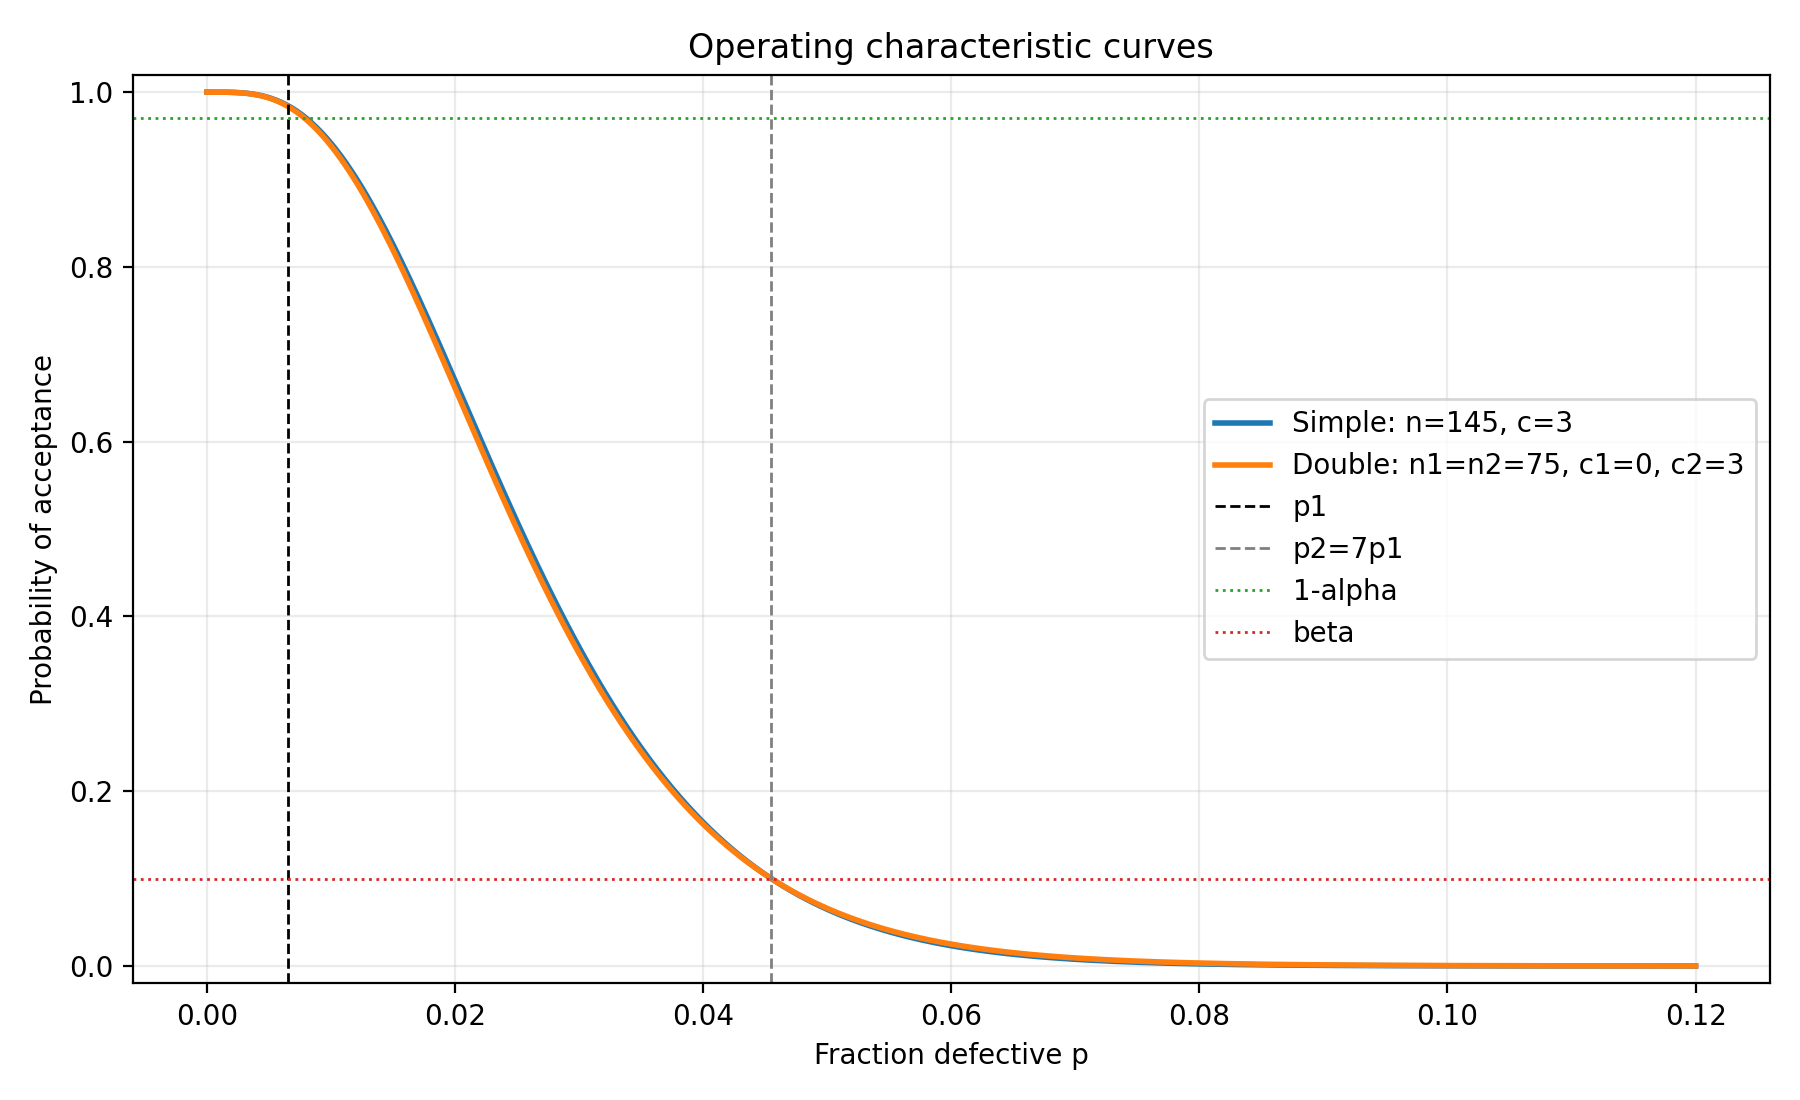
\includegraphics[width=0.92\textwidth]{acceptance_oc_curves.png}
\caption{Καμπύλες χαρακτηριστικής αποδοχής για το απλό και το διπλό σχήμα.}
\label{fig:oc}
\end{figure}

\subsubsection*{Καμπύλες ATI}

Στο Σχήμα~\ref{fig:ati} φαίνονται οι \(\ATI(p)\). Εδώ η διαφορά μεταξύ απλού
και διπλού σχήματος είναι ορατή.

\begin{figure}[H]
\centering
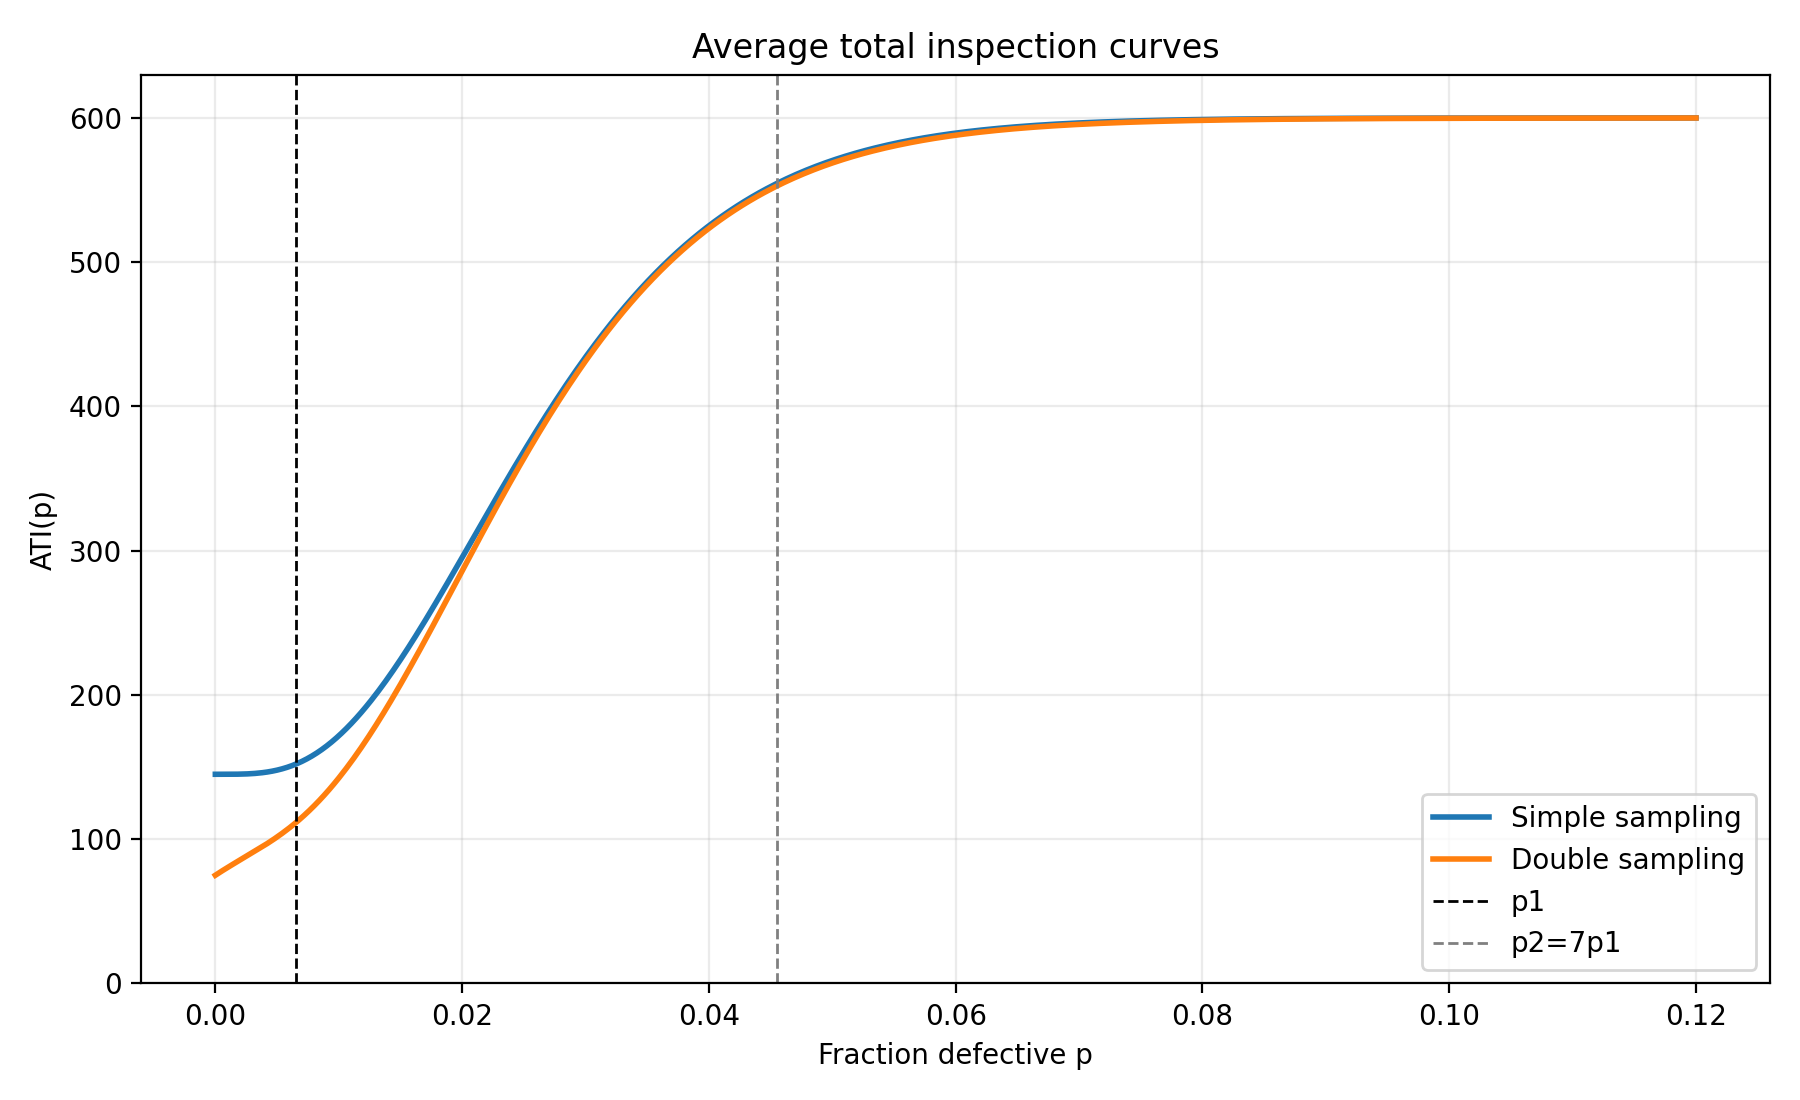
\includegraphics[width=0.92\textwidth]{acceptance_ati_curves.png}
\caption{Μέσος συνολικός αριθμός επιθεωρούμενων μονάδων για κάθε σχήμα.}
\label{fig:ati}
\end{figure}

Για πολύ μικρά \(p\), η καμπύλη του διπλού σχήματος είναι χαμηλότερα. Αυτό
σημαίνει ότι ελέγχονται λιγότερες μονάδες κατά μέσο όρο. Πολλές παρτίδες
αποδέχονται από το πρώτο δείγμα 75 μονάδων και δεν χρειάζεται δεύτερο.

Καθώς το \(p\) αυξάνεται, οι απορρίψεις αυξάνονται, οπότε γίνεται όλο και
συχνότερα ο 100\% έλεγχος. Έτσι και οι δύο καμπύλες ανεβαίνουν προς το
\(N=600\).

\subsubsection*{Καμπύλες AOQ}

Στο Σχήμα~\ref{fig:aoq} φαίνονται οι \(\AOQ(p)\). Και οι δύο μένουν κάτω από
την κόκκινη οριζόντια γραμμή \(3p_1=0{,}0195\). Αυτό επιβεβαιώνει ότι ο
περιορισμός του \(\AOQL\) ικανοποιείται.

\begin{figure}[H]
\centering
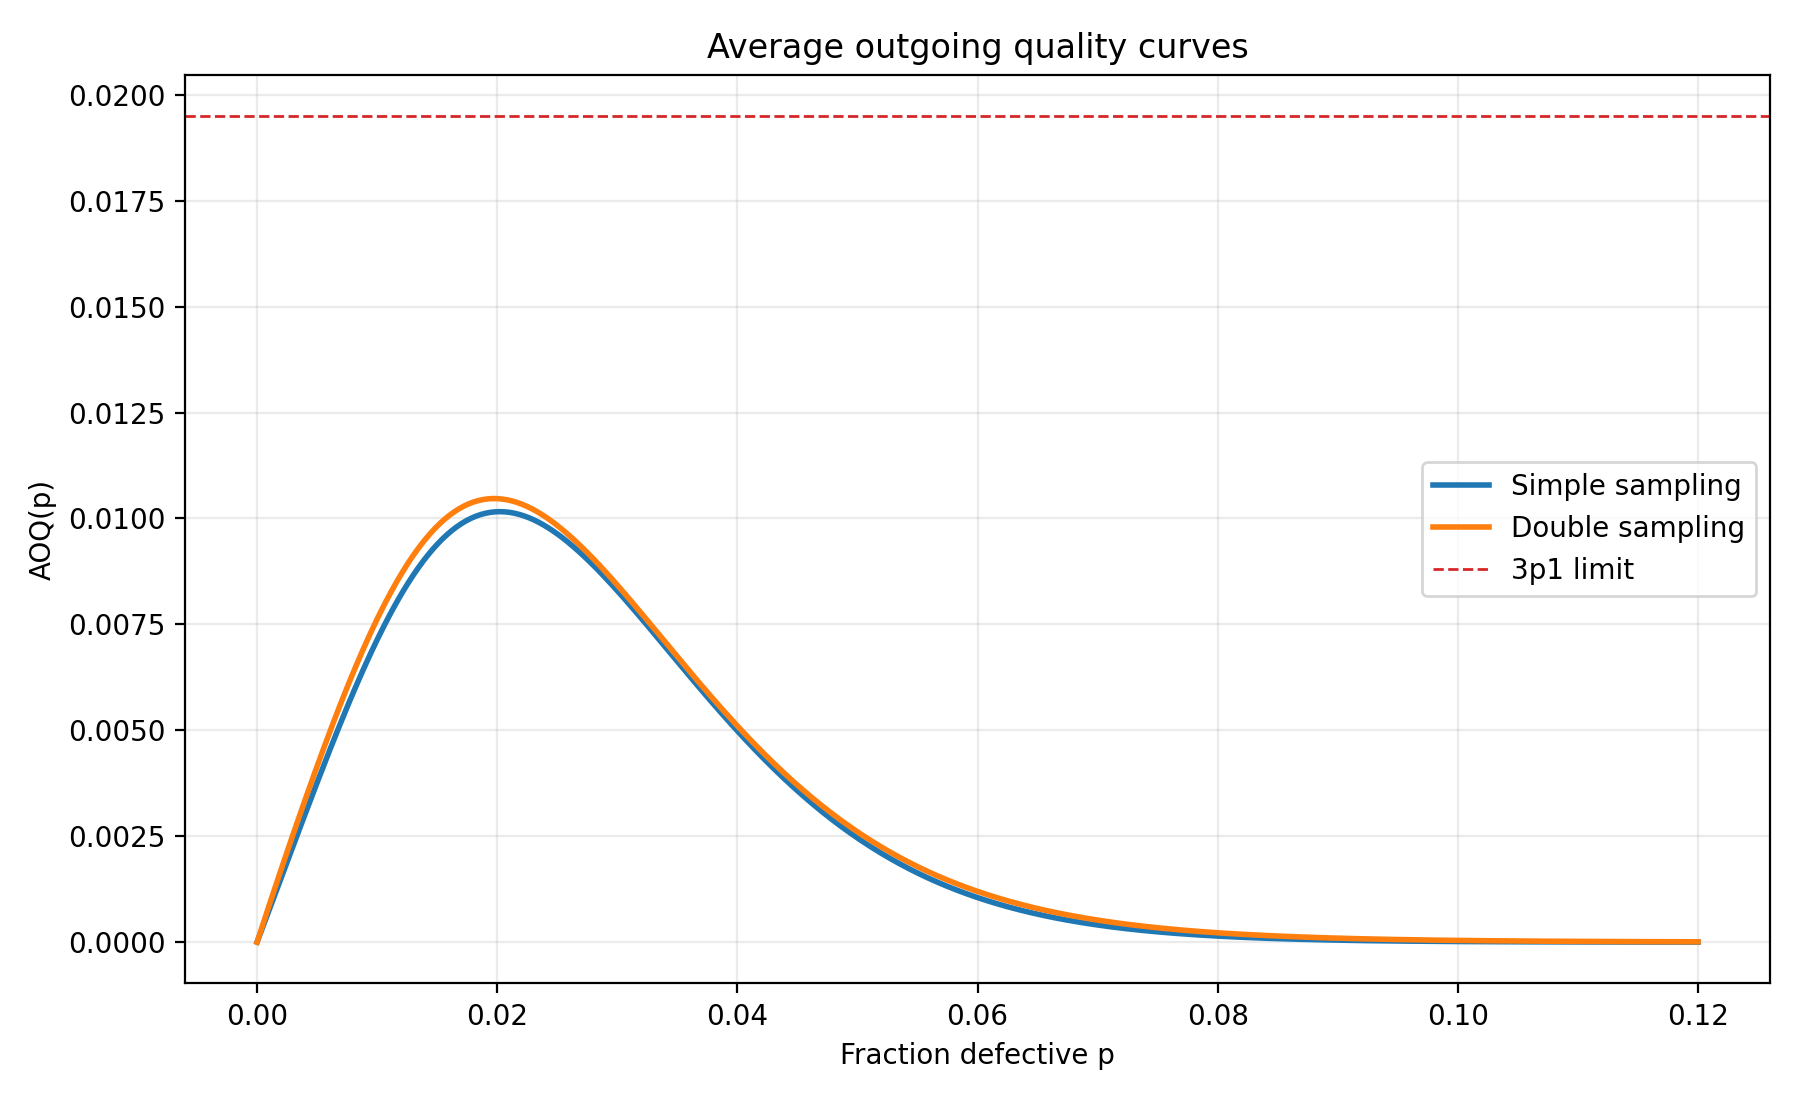
\includegraphics[width=0.92\textwidth]{acceptance_aoq_curves.png}
\caption{Μέση εξερχόμενη ποιότητα συναρτήσει του \(p\), και το όριο \(3p_1\).}
\label{fig:aoq}
\end{figure}

\subsubsection*{Πρακτικό συμπέρασμα Α3}

Τα δύο σχήματα έχουν παρόμοια ικανότητα διάκρισης καλών και κακών παρτίδων.
Το διπλό σχήμα έχει το πλεονέκτημα ότι όταν η ποιότητα είναι όντως καλή,
ελέγχει λιγότερες μονάδες. Όταν όμως η ποιότητα είναι κακή, και τα δύο
σχήματα οδηγούνται σε σχεδόν πλήρη έλεγχο.

%-----------------------------------------------------------------------------
\subsection{Ερώτημα Α4: Οικονομικά βέλτιστο απλό σχήμα}
%-----------------------------------------------------------------------------

\subsubsection*{Τι ζητάει το ερώτημα}

Αλλάζει εντελώς το κριτήριο. Δεν μας ενδιαφέρουν πια οι κίνδυνοι παραγωγού
και πελάτη ως απαιτήσεις. Θέλουμε να βρούμε απλό σχήμα που \emph{ελαχιστοποιεί
το μέσο συνολικό κόστος} ανά παρτίδα, με τον περιορισμό \(c\le 1\).

Επιπλέον, η εκφώνηση μας λέει ότι το \(p\) δεν είναι σταθερό. Είναι τυχαία
μεταβλητή με ομοιόμορφη κατανομή στο διάστημα \([p_L,p_U]=[0{,}004,\,0{,}060]\).

\begin{intuition}
``Ομοιόμορφη'' σημαίνει ότι κάθε τιμή του \(p\) μέσα στο διάστημα είναι
εξίσου πιθανή. Δεν περιμένουμε ούτε ότι θα είναι χαμηλό, ούτε ότι θα είναι
ψηλό. Όλες οι τιμές είναι ισότιμα πιθανές. Σαν να ρίχνουμε ένα ζάρι που
γράφει τιμές μεταξύ 0,004 και 0,060.
\end{intuition}

\subsubsection*{Δομή του κόστους}

Το συνολικό κόστος ανά παρτίδα έχει δύο συνιστώσες:

\textbf{Κόστος ελέγχου:} ο μέσος αριθμός ελεγχόμενων μονάδων είναι \(\ATI(p)\)
και κάθε μονάδα κοστίζει \(c_i\). Άρα:
\[
    C_{\text{έλεγχος}}(p)=c_i\,\ATI(p).
\]

\textbf{Κόστος διαφυγής:} όσα ελαττωματικά ξεγλιστρούν στον πελάτη κοστίζουν
\(c_d\) το καθένα. Ο μέσος αριθμός τους είναι:
\[
    \text{Escaped}(p)=p\,\Pa(p)\,(N-n).
\]

Άρα το συνολικό κόστος για δεδομένο \(p\) είναι:
\[
    C(p)=c_i\,\ATI(p)+c_d\,p\,\Pa(p)\,(N-n).
\]

\begin{trap}
Μην ξεχάσετε το \((N-n)\) στο δεύτερο όρο. Είναι ο αριθμός μονάδων εκτός
δείγματος. Μόνο αυτές μπορούν να ξεγλιστρήσουν στον πελάτη.
\end{trap}

\subsubsection*{Μέσο κόστος όταν το \(p\) είναι τυχαίο}

Επειδή το \(p\) είναι τυχαίο ομοιόμορφο, παίρνουμε το μέσο όρο ως προς \(p\):
\[
    E[C]=\frac{1}{p_U-p_L}\int_{p_L}^{p_U}C(p)\,dp.
\]

Σε υπολογιστική γλώσσα, αυτό είναι αριθμητική ολοκλήρωση. Η Python το κάνει
με τη συνάρτηση \code{scipy.integrate.quad}.

\subsubsection*{Αλγόριθμος αναζήτησης}

\begin{enumerate}[leftmargin=2.2em]
    \item Για κάθε \(n\) από 1 έως 600 και για κάθε \(c\in\{0,1\}\), υπολογίζουμε
    το \(E[C]\).
    \item Καταγράφουμε όλα τα ζεύγη και ταξινομούμε αύξουσα ως προς το κόστος.
    \item Παίρνουμε το ζεύγος με το μικρότερο κόστος.
\end{enumerate}

Το αποτέλεσμα είναι:
\[
    \boxed{n=189,\quad c=1}.
\]

Δηλαδή:

\begin{itemize}[leftmargin=2.2em]
    \item Παίρνουμε δείγμα 189 εξαρτημάτων.
    \item Αποδεχόμαστε αν βρούμε 0 ή 1 ελαττωματικό.
    \item Απορρίπτουμε διαφορετικά.
\end{itemize}

\begin{table}[H]
\centering
\caption{Σύγκριση μέσου συνολικού κόστους.}
\begin{tabular}{lrrr}
\toprule
\textbf{Σχήμα} & \textbf{\(n\)} & \textbf{\(c\)} & \textbf{Μέσο κόστος} \\
\midrule
Βέλτιστο με \(c\le 1\) & 189 & 1 & 3.522,36 € \\
Σχήμα Ερωτήματος Α1   & 145 & 3 & 3.912,03 € \\
\bottomrule
\end{tabular}
\end{table}

Η διαφορά είναι:
\[
    3.912{,}03-3.522{,}36=389{,}67 \text{ € ανά παρτίδα},
\]
δηλαδή το σχήμα του Α1 είναι περίπου 11\% πιο ακριβό με αυτό το κριτήριο.

\begin{intuition}
Γιατί το οικονομικά βέλτιστο σχήμα έχει \emph{μεγαλύτερο} \(n\) και
\emph{μικρότερο} \(c\); Επειδή τώρα ψάχνουμε ισορροπία ανάμεσα σε δύο
κόστη. Όταν \(n\) μεγαλώνει, ελέγχω περισσότερες μονάδες, οπότε λιγότερες
έχουν ευκαιρία να ξεφύγουν. Το ίδιο πετυχαίνω και με αυστηρότερο \(c\)
(μικρότερη ανοχή). Ο αλγόριθμος διάλεξε αυτόν τον συνδυασμό γιατί ταιριάζει
καλύτερα στις σχετικές τιμές \(c_i=6\) και \(c_d=400\).
\end{intuition}

\begin{trap}
Δεν είναι σωστό να πούμε ότι ``το σχήμα του Α1 ήταν λάθος''. Το Α1 σχεδιάστηκε
να ικανοποιεί στατιστικές απαιτήσεις (κίνδυνους και \(\AOQL\)), όχι να
ελαχιστοποιεί κόστος. Είναι δύο διαφορετικές βελτιστοποιήσεις. Κάθε μία έχει
νόημα στο δικό της πλαίσιο.
\end{trap}

\newpage

%=============================================================================
\section{Στατιστικά θεμέλια του Μέρους Β}
%=============================================================================

Το Μέρος Β χρησιμοποιεί κανονική κατανομή. Συγκεντρώνουμε εδώ όλα τα
απαραίτητα στατιστικά εργαλεία πριν τα εφαρμόσουμε στα ερωτήματα.

\subsection{Η κανονική κατανομή με απλά λόγια}

Όταν η τάση εξόδου μετρηθεί σε ένα τυχαία επιλεγμένο τροφοδοτικό, παίρνει
μια τιμή λίγο διαφορετική κάθε φορά. Αν η διαδικασία λειτουργεί σταθερά, οι
τιμές διασκορπίζονται γύρω από μια μέση τιμή \(\mu_0\) με τυπική απόκλιση
\(\sigma\). Λέμε:
\[
    X\sim N(\mu_0,\sigma^2).
\]

Πρακτικά:

\begin{itemize}[leftmargin=2.2em]
    \item Περίπου 68\% των τιμών πέφτουν μέσα στο \(\mu_0\pm \sigma\).
    \item Περίπου 95\% πέφτουν μέσα στο \(\mu_0\pm 2\sigma\).
    \item Περίπου 99,7\% πέφτουν μέσα στο \(\mu_0\pm 3\sigma\).
\end{itemize}

\begin{intuition}
Φανταστείτε ότι ρίχνετε χιλιάδες σταγόνες χρώμα γύρω από ένα κέντρο. Αν δεν
υπάρχει συστηματική απόκλιση, τα περισσότερα χτυπήματα είναι στο κέντρο και
γίνονται όλο και πιο λίγα όσο απομακρυνόμαστε. Αυτή η εικόνα είναι η
κανονική καμπύλη.
\end{intuition}

\subsection{Κατανομή της δειγματικής μέσης τιμής}

Αν παίρνουμε δείγμα μεγέθους \(n\) από \(N(\mu_0,\sigma^2)\), η δειγματική
μέση τιμή \(\bar X\) ακολουθεί:
\[
    \bar X\sim N\!\left(\mu_0,\frac{\sigma^2}{n}\right).
\]

Δηλαδή έχει την ίδια μέση τιμή, αλλά μικρότερη τυπική απόκλιση. Συγκεκριμένα:
\[
    \sigma_{\bar X}=\frac{\sigma}{\sqrt n}.
\]

\begin{intuition}
Η μέση τιμή ενός δείγματος είναι πιο ``σταθερή'' από μια μεμονωμένη μέτρηση,
γιατί οι θετικές και αρνητικές μικρές αποκλίσεις τείνουν να αλληλοεξουδετερώνονται
στο μέσο όρο.
\end{intuition}

\subsection{Κατανομή της δειγματικής τυπικής απόκλισης}

Για κανονικά δεδομένα, το \(S\) έχει \emph{αναμενόμενη τιμή} λίγο μικρότερη
από \(\sigma\). Συγκεκριμένα:
\[
    E[S]=c_4\,\sigma,
\]
όπου:
\[
    c_4=\sqrt{\frac{2}{n-1}}\,\frac{\Gamma(n/2)}{\Gamma((n-1)/2)}.
\]

Ο \(c_4\) διορθώνει αυτή τη μικρή απόκλιση. Για \(n=5\) (όπως στην εργασία):
\[
    c_4=0{,}939986.
\]

Η τυπική απόκλιση του ίδιου του \(S\) είναι:
\[
    \sigma_S=\sigma\sqrt{1-c_4^2}.
\]

Επίσης, για κανονικά δεδομένα ισχύει:
\[
    \frac{(n-1)S^2}{\sigma^2}\sim\chi^2_{n-1}.
\]

Αυτή η τελευταία σχέση θα μας επιτρέψει να υπολογίζουμε ακριβείς πιθανότητες
για το \(S\) σαν αυτές που χρειάζονται στα διαγράμματα.

\begin{intuition}
Η κατανομή \(\chi^2\) (χι-τετράγωνο) είναι ένας τρόπος να μετράμε πόσο
``διασκορπισμένα'' είναι τα δείγματά μας. Όσο μεγαλύτερη μεταβλητότητα, τόσο
μεγαλύτερες τιμές παίρνει.
\end{intuition}

\subsection{Διαγράμματα ελέγχου: τι είναι και γιατί υπάρχουν}

Ένα διάγραμμα ελέγχου είναι ένα διάγραμμα στον χρόνο. Στον οριζόντιο άξονα
έχουμε τη στιγμή κάθε δείγματος. Στον κατακόρυφο άξονα έχουμε ένα στατιστικό
μέγεθος του δείγματος, π.χ. τη μέση τιμή ή την τυπική απόκλιση.

Πάνω από και κάτω από το κεντρικό όριο σχεδιάζουμε δύο όρια, τα όρια ελέγχου.
Όσο η διαδικασία λειτουργεί κανονικά, τα δειγματικά μεγέθη μένουν εντός των
ορίων. Αν κάποιο πάει εκτός ορίων, αυτό είναι ένδειξη ότι κάτι στη διαδικασία
άλλαξε.

\begin{intuition}
Σκεφτείτε τον γιατρό που μετράει πίεση κάθε εβδομάδα. Αν η μέτρηση είναι κάθε
φορά γύρω στα 12, τότε όλα είναι ήρεμα. Αν ξαφνικά γίνει 17, ο γιατρός
αναρωτιέται αν κάτι έχει αλλάξει. Τα όρια ελέγχου παίζουν τον ρόλο του ``πότε
πρέπει να αναρωτηθούμε''.
\end{intuition}

\subsection{Σφάλμα τύπου Ι, σφάλμα τύπου ΙΙ και ισχύς}

Σε κάθε στατιστικό σύστημα ελέγχου μπορούν να συμβούν δύο είδη σφαλμάτων:

\begin{itemize}[leftmargin=2.2em]
    \item \textbf{Σφάλμα τύπου Ι (\(\alpha\)).} Δίνουμε σήμα ``εκτός ελέγχου''
    ενώ στην πραγματικότητα η διαδικασία είναι κανονική. Είναι ψευδής συναγερμός.
    \item \textbf{Σφάλμα τύπου ΙΙ (\(\beta\)).} Δεν δίνουμε σήμα, ενώ στην
    πραγματικότητα έχει συμβεί αλλαγή. Είναι ``το προσπεράσαμε''.
\end{itemize}

Η \emph{ισχύς} του διαγράμματος είναι η πιθανότητα να πιάσει την αλλαγή,
δηλαδή:
\[
    \text{ισχύς}=1-\beta.
\]

\subsection{Average Run Length (ARL)}

Αν σε κάθε δείγμα η πιθανότητα ένδειξης είναι \(\pi\), τότε ο μέσος αριθμός
δειγμάτων μέχρι να εμφανιστεί η πρώτη ένδειξη είναι:
\[
    \ARL=\frac{1}{\pi}.
\]

Όταν η διαδικασία είναι εντός ελέγχου, χρησιμοποιούμε το \(\ARL_0=1/\alpha\).
Είναι ο μέσος αριθμός δειγμάτων μέχρι έναν ψευδή συναγερμό.

Όταν η διαδικασία είναι εκτός ελέγχου, χρησιμοποιούμε το \(\ARL_1\). Είναι ο
μέσος αριθμός δειγμάτων μέχρι να καταλάβουμε την αλλαγή.

\newpage

%=============================================================================
\section{Μέρος Β: Διαγράμματα ελέγχου}
%=============================================================================

\subsection{Γενική εικόνα του Μέρους Β}

Έχουμε μια γραμμή παραγωγής τροφοδοτικών που λειτουργεί συνεχώς. Κάθε ώρα
παίρνουμε δείγμα 5 τροφοδοτικών και μετράμε την τάση εξόδου του καθενός.
Από αυτές τις 5 μετρήσεις υπολογίζουμε δύο μεγέθη:

\begin{itemize}[leftmargin=2.2em]
    \item τη δειγματική μέση τιμή \(\bar X\),
    \item τη δειγματική τυπική απόκλιση \(S\).
\end{itemize}

Φτιάχνουμε δύο ξεχωριστά διαγράμματα, ένα για το \(\bar X\) και ένα για το
\(S\). Παρακολουθούμε και τα δύο.

\begin{intuition}
Με το διάγραμμα \(\bar X\) ελέγχουμε αν το ``κέντρο'' της παραγωγής έχει
μετατοπιστεί. Με το διάγραμμα \(S\) ελέγχουμε αν η ``διασπορά'' της
παραγωγής έχει μεγαλώσει. Είναι σαν δύο διαφορετικοί αισθητήρες που
δουλεύουν παράλληλα.
\end{intuition}

%-----------------------------------------------------------------------------
\subsection{Ερώτημα Β1: Κατασκευή των διαγραμμάτων}
%-----------------------------------------------------------------------------

\subsubsection*{Τι ζητάει το ερώτημα}

Να υπολογίσουμε τα τρία όρια κάθε διαγράμματος: \(LCL\), \(CL\), \(UCL\).
Χρησιμοποιούμε όρια \(k=2{,}5\) τυπικών αποκλίσεων.

\subsubsection*{Διάγραμμα \(\bar X\)}

Η δειγματική μέση τιμή έχει τυπική απόκλιση \(\sigma/\sqrt n\), άρα τα όρια
βρίσκονται \(k\) τέτοιες αποκλίσεις γύρω από \(\mu_0\):
\[
    LCL_{\bar X}=\mu_0-k\frac{\sigma}{\sqrt n},\quad
    CL_{\bar X}=\mu_0,\quad
    UCL_{\bar X}=\mu_0+k\frac{\sigma}{\sqrt n}.
\]

Με \(\mu_0=9\), \(\sigma=0{,}035\), \(n=5\), \(k=2{,}5\) υπολογίζουμε
βήμα προς βήμα:

\textbf{Βήμα 1.} Τυπική απόκλιση της \(\bar X\):
\[
    \frac{\sigma}{\sqrt n}=\frac{0{,}035}{\sqrt 5}=\frac{0{,}035}{2{,}23607}=0{,}015652.
\]

\textbf{Βήμα 2.} Πολλαπλασιάζουμε με \(k\):
\[
    2{,}5\times 0{,}015652=0{,}039131.
\]

\textbf{Βήμα 3.} Αφαιρούμε και προσθέτουμε στο \(\mu_0\):
\[
    LCL_{\bar X}=9-0{,}039131=8{,}960869,
\]
\[
    UCL_{\bar X}=9+0{,}039131=9{,}039131.
\]

\subsubsection*{Διάγραμμα \(S\)}

Το διάγραμμα \(S\) δεν είναι συμμετρικό. Το κεντρικό όριο δεν είναι το
\(\sigma\), αλλά:
\[
    CL_S=c_4\sigma.
\]

Τα όρια ορίζονται με την τυπική απόκλιση του ίδιου του \(S\):
\[
    \sigma_S=\sigma\sqrt{1-c_4^2}.
\]

Άρα:
\[
    LCL_S=\max(0,\,c_4\sigma-k\sigma_S),
\]
\[
    UCL_S=c_4\sigma+k\sigma_S.
\]

\begin{intuition}
Ο όρος \(\max(0,\ldots)\) χρειάζεται επειδή η τυπική απόκλιση δεν μπορεί να
γίνει αρνητική. Αν ο τύπος μας έδινε αρνητικό κάτω όριο, θα έπρεπε να το
αντικαταστήσουμε με μηδέν.
\end{intuition}

Βήμα προς βήμα:

\textbf{Βήμα 1.} Υπολογίζουμε το \(c_4\) για \(n=5\):
\[
    c_4=\sqrt{\frac{2}{4}}\,\frac{\Gamma(2{,}5)}{\Gamma(2)}
    =0{,}939986.
\]

\textbf{Βήμα 2.} Κεντρικό όριο:
\[
    CL_S=0{,}939986\times 0{,}035=0{,}032899.
\]

\textbf{Βήμα 3.} Τυπική απόκλιση του \(S\):
\[
    \sigma_S=0{,}035\times\sqrt{1-(0{,}939986)^2}=0{,}035\times 0{,}341227=0{,}011943.
\]

\textbf{Βήμα 4.} Πολλαπλασιάζουμε με \(k\):
\[
    2{,}5\times 0{,}011943=0{,}029856.
\]

\textbf{Βήμα 5.} Όρια:
\[
    LCL_S=\max(0,\,0{,}032899-0{,}029856)=0{,}003043,
\]
\[
    UCL_S=0{,}032899+0{,}029856=0{,}062756.
\]

\begin{table}[H]
\centering
\caption{Τελικά όρια των διαγραμμάτων ελέγχου.}
\begin{tabular}{lrrr}
\toprule
\textbf{Διάγραμμα} & \textbf{LCL} & \textbf{CL} & \textbf{UCL} \\
\midrule
\(\bar X\) & 8,960869 & 9,000000 & 9,039131 \\
\(S\) & 0,003043 & 0,032899 & 0,062756 \\
\bottomrule
\end{tabular}
\end{table}

%-----------------------------------------------------------------------------
\subsection{Ερώτημα Β2: Πιθανότητα σφάλματος πρώτου είδους}
%-----------------------------------------------------------------------------

\subsubsection*{Τι ζητάει το ερώτημα}

Όταν η διαδικασία είναι κανονική, πόσο συχνά θα μας δίνει ψευδή συναγερμό
τουλάχιστον ένα από τα δύο διαγράμματα; Αυτό είναι το συνολικό σφάλμα
τύπου Ι.

\subsubsection*{Σφάλμα τύπου Ι του \(\bar X\)}

Όταν η διαδικασία είναι εντός ελέγχου:
\[
    \bar X\sim N(\mu_0,\sigma^2/n).
\]

Άρα η τυποποιημένη μεταβλητή:
\[
    Z=\frac{\bar X-\mu_0}{\sigma/\sqrt n}\sim N(0,1).
\]

Τα όρια απέχουν \(k=2{,}5\) τυπικές αποκλίσεις από το \(\mu_0\). Άρα:
\[
    \alpha_{\bar X}=P(|Z|>2{,}5)=2\bigl(1-\Phi(2{,}5)\bigr).
\]

Με \(\Phi(2{,}5)=0{,}993790\):
\[
    \alpha_{\bar X}=2(1-0{,}993790)=2\times 0{,}006210=0{,}012419.
\]

\subsubsection*{Σφάλμα τύπου Ι του \(S\)}

Όταν η διαδικασία είναι εντός ελέγχου:
\[
    \frac{(n-1)S^2}{\sigma^2}\sim\chi^2_{n-1}=\chi^2_4.
\]

Άρα:
\[
    P(S<LCL_S)=P\!\left(\chi^2_4<\frac{(n-1)LCL_S^2}{\sigma^2}\right),
\]
\[
    P(S>UCL_S)=P\!\left(\chi^2_4>\frac{(n-1)UCL_S^2}{\sigma^2}\right).
\]

Χρησιμοποιούμε τη συνάρτηση \code{chi2.cdf} της Python και προκύπτει:
\[
    \alpha_S=0{,}012095.
\]

\subsubsection*{Συνολικό σφάλμα τύπου Ι}

Επειδή για κανονικά δεδομένα οι \(\bar X\) και \(S\) είναι ανεξάρτητα, η
πιθανότητα κανένα διάγραμμα να μη δώσει σήμα είναι:
\[
    (1-\alpha_{\bar X})(1-\alpha_S).
\]

Άρα η πιθανότητα τουλάχιστον ένα διάγραμμα να δώσει ψευδή ένδειξη είναι:
\[
    \alpha_{\text{ολ}}=1-(1-\alpha_{\bar X})(1-\alpha_S).
\]

Υπολογισμός:
\[
    (1-0{,}012419)(1-0{,}012095)=0{,}987581\times 0{,}987905=0{,}975636,
\]
\[
    \alpha_{\text{ολ}}=1-0{,}975636=0{,}024364.
\]

\[
    \boxed{\alpha_{\text{ολ}}=0{,}024364}.
\]

Δηλαδή σε κάθε ωριαία δειγματοληψία, ακόμη και αν όλα είναι εντάξει, υπάρχει
περίπου 2,44\% πιθανότητα να σταματήσουμε άσκοπα τη διαδικασία.

\begin{intuition}
Το \(\ARL_0=1/0{,}024364\approx 41\) σημαίνει ότι αν η διαδικασία είναι
απολύτως κανονική, κατά μέσο όρο κάθε 41 δείγματα (δηλαδή 41 ώρες) θα
έχουμε ένα ψευδή συναγερμό. Αν θεωρούμε ότι αυτό είναι πάρα πολύ συχνό,
μπορούμε να ανοίξουμε τα όρια. Αν είναι λίγο, μπορούμε να τα στενέψουμε.
\end{intuition}

%-----------------------------------------------------------------------------
\subsection{Ερώτημα Β3: Ισχύς του διαγράμματος μέσης τιμής}
%-----------------------------------------------------------------------------

\subsubsection*{Τι ζητάει το ερώτημα}

Αν η μέση τιμή της διαδικασίας μετατοπιστεί κατά \(\Delta=0{,}06\), δηλαδή
γίνει \(9{,}06\) (ή \(8{,}94\)), τι πιθανότητα έχει το διάγραμμα \(\bar X\)
να το πιάσει με την επόμενη κιόλας δειγματοληψία;

Δύο περιπτώσεις:

\begin{enumerate}[leftmargin=2.2em]
    \item Μεταβολή μέσης τιμής, η τυπική απόκλιση μένει \(\sigma\).
    \item Μεταβολή μέσης τιμής, και ταυτόχρονα η τυπική απόκλιση γίνεται
    \(1{,}2\sigma\).
\end{enumerate}

\subsubsection*{Θεωρητικός υπολογισμός}

Αν η νέα κατάσταση είναι \(\bar X\sim N(\mu_1,\sigma'^2/n)\), τότε:
\[
    \text{ισχύς}=P(\bar X<LCL_{\bar X})+P(\bar X>UCL_{\bar X}).
\]

Λόγω συμμετρίας, η μετατόπιση κατά \(+\Delta\) δίνει την ίδια ισχύ με τη
μετατόπιση κατά \(-\Delta\).

\subsubsection*{Περίπτωση 1: μετατόπιση χωρίς αύξηση \(\sigma\)}

\(\mu_1=9{,}06\), \(\sigma'=0{,}035\), τυπική απόκλιση της \(\bar X\):
\[
    \frac{\sigma'}{\sqrt n}=0{,}015652.
\]

Υπολογίζουμε δύο πιθανότητες:
\[
    P(\bar X<8{,}960869)\quad\text{με κατανομή}\quad N(9{,}06,\,0{,}015652^2),
\]
\[
    P(\bar X>9{,}039131)\quad\text{με την ίδια κατανομή}.
\]

Από τους τύπους της κανονικής:
\[
    \text{ισχύς}\approx 0{,}908777.
\]

\[
    \boxed{0{,}908777}.
\]

\subsubsection*{Περίπτωση 2: μετατόπιση και ταυτόχρονη αύξηση \(\sigma\)}

Τώρα \(\sigma'=1{,}2\sigma=0{,}042\), άρα τυπική απόκλιση της \(\bar X\):
\[
    \frac{0{,}042}{\sqrt 5}=0{,}018782.
\]

Με ανάλογους υπολογισμούς:
\[
    \text{ισχύς}\approx 0{,}866727.
\]

\[
    \boxed{0{,}866727}.
\]

\begin{table}[H]
\centering
\caption{Ισχύς του διαγράμματος \(\bar X\).}
\begin{tabular}{lr}
\toprule
\textbf{Περίπτωση} & \textbf{Ισχύς} \\
\midrule
Μεταβολή μέσης τιμής, χωρίς αύξηση \(\sigma\) & 0,908777 \\
Μεταβολή μέσης τιμής, με αύξηση \(\sigma\) κατά 20\% & 0,866727 \\
\bottomrule
\end{tabular}
\end{table}

\begin{intuition}
Η μετατόπιση \(0{,}06\) είναι σχεδόν \(\Delta/\sigma_{\bar X}=3{,}83\) τυπικές
αποκλίσεις της \(\bar X\). Είναι μεγάλη σε στατιστικούς όρους, γι' αυτό η
ισχύς είναι πολύ ψηλή. Όταν η μεταβλητότητα αυξάνεται 20\%, η κατανομή της
\(\bar X\) απλώνεται, οπότε λίγες περισσότερες τιμές παραμένουν εντός ορίων.
\end{intuition}

%-----------------------------------------------------------------------------
\subsection{Ερώτημα Β4: Ισχύς του διαγράμματος τυπικής απόκλισης}
%-----------------------------------------------------------------------------

\subsubsection*{Τι ζητάει το ερώτημα}

Αν η τυπική απόκλιση αυξηθεί από \(\sigma\) σε \(1{,}2\sigma\), πόσο γρήγορα
θα το πιάσει το διάγραμμα \(S\); Και τι αλλάζει αν ταυτόχρονα έχουμε και
μετατόπιση της μέσης τιμής;

\subsubsection*{Κρίσιμη παρατήρηση}

Η κατανομή του \(S\) εξαρτάται μόνο από τη \(\sigma\) και όχι από τη μέση
τιμή \(\mu\). Αυτό φαίνεται από το γεγονός ότι:
\[
    \frac{(n-1)S^2}{\sigma^2}\sim\chi^2_{n-1},
\]
χωρίς το \(\mu\) να εμφανίζεται πουθενά. Άρα αν μόνο η μέση τιμή αλλάξει,
το \(S\) δεν μπορεί να το αντιληφθεί.

\subsubsection*{Υπολογισμός}

Με νέα τυπική απόκλιση \(\sigma'=1{,}2\sigma=0{,}042\):
\[
    \text{ισχύς}=P\!\left(\chi^2_4<\frac{4\cdot LCL_S^2}{\sigma'^2}\right)
    + P\!\left(\chi^2_4>\frac{4\cdot UCL_S^2}{\sigma'^2}\right).
\]

Προκύπτει:
\[
    \boxed{0{,}062919}.
\]

Αυτό σημαίνει ότι μόνο περίπου 6,3\% πιθανότητα έχει το διάγραμμα \(S\) να
πιάσει την αύξηση της μεταβλητότητας στην επόμενη δειγματοληψία.

\begin{table}[H]
\centering
\caption{Ισχύς του διαγράμματος \(S\).}
\begin{tabular}{lr}
\toprule
\textbf{Περίπτωση} & \textbf{Ισχύς} \\
\midrule
Αύξηση \(\sigma\) κατά 20\%, χωρίς μεταβολή \(\mu\) & 0,062919 \\
Αύξηση \(\sigma\) κατά 20\%, με μεταβολή \(\mu\) & 0,062919 \\
\bottomrule
\end{tabular}
\end{table}

\begin{intuition}
Η ισχύς του \(S\) είναι μικρή για δύο λόγους: τα όρια είναι αρκετά πλατιά
(\(k=2{,}5\)) και το μέγεθος δείγματος είναι μικρό (\(n=5\)). Αν θέλαμε
ευαισθησία, θα μπορούσαμε να αυξήσουμε το \(n\) ή να μειώσουμε το \(k\), με
το τίμημα όμως περισσότερων ψευδών συναγερμών.
\end{intuition}

%-----------------------------------------------------------------------------
\subsection{Ερώτημα Β5: Κόστος κακής ποιότητας μέχρι την ανίχνευση}
%-----------------------------------------------------------------------------

\subsubsection*{Τι ζητάει το ερώτημα}

Έστω ότι η μέση τιμή μετατοπίζεται από 9 σε 9,06. Όσο η μετατόπιση δεν έχει
ανιχνευθεί, η διαδικασία παράγει ελαττωματικά τροφοδοτικά (δηλαδή τάση εκτός
\([8{,}90,\,9{,}10]\)) με αυξημένη πιθανότητα. Πόσο μας στοιχίζει αυτό
οικονομικά, μέχρι το διάγραμμα να δώσει ένδειξη;

Η τυπική απόκλιση θεωρείται αμετάβλητη.

\subsubsection*{Βήμα 1: Πιθανότητα ελαττωματικού μετά τη μετατόπιση}

Με νέα κατανομή \(X\sim N(9{,}06,\,0{,}035^2)\):
\[
    P(X<8{,}90)=\Phi\!\left(\frac{8{,}90-9{,}06}{0{,}035}\right)=\Phi(-4{,}571)\approx 2{,}4\cdot 10^{-6},
\]
\[
    P(X>9{,}10)=1-\Phi\!\left(\frac{9{,}10-9{,}06}{0{,}035}\right)=1-\Phi(1{,}143)\approx 0{,}12655.
\]

Άθροισμα:
\[
    P(\text{ελαττωματικό})\approx 0{,}126551.
\]

\subsubsection*{Βήμα 2: Κόστος ανά ώρα ενώ η διαδικασία είναι μετατοπισμένη}

Η παραγωγή είναι 100 τροφοδοτικά την ώρα. Κάθε ελαττωματικό στοιχίζει
\(K=21\) €. Άρα:
\[
    C_{\text{ώρα}}=0{,}126551\times 100\times 21=265{,}76 \text{ €/ώρα}.
\]

\subsubsection*{Βήμα 3: Πόσος χρόνος μέχρι ανίχνευση}

Η πιθανότητα ανίχνευσης σε κάθε δείγμα είναι η ισχύς του \(\bar X\) από το
Β3:
\[
    \pi=0{,}908777.
\]

Άρα ο μέσος αριθμός δειγμάτων μέχρι την ένδειξη είναι:
\[
    \ARL_1=\frac{1}{0{,}908777}=1{,}10038.
\]

Δύο σενάρια για τη χρονική στιγμή που συμβαίνει η μετατόπιση:

\begin{itemize}[leftmargin=2.2em]
    \item \textbf{Αμέσως μετά από δειγματοληψία.} Πρέπει να περιμένουμε όλον
    τον κύκλο μέχρι το επόμενο δείγμα. Άρα ο μέσος χρόνος είναι
    \(\ARL_1\) ώρες.
    \item \textbf{Σε τυχαία στιγμή μέσα στο ωριαίο διάστημα.} Κατά μέσο όρο
    χάνουμε μισή ώρα λιγότερη. Άρα ο μέσος χρόνος είναι \(\ARL_1-1/2\) ώρες.
\end{itemize}

Με αριθμούς:
\[
    \text{Σενάριο Α: } 1{,}10038 \text{ ώρες,}
\]
\[
    \text{Σενάριο Β: } 1{,}10038-0{,}5=0{,}60038 \text{ ώρες.}
\]

\subsubsection*{Βήμα 4: Συνολικό μέσο κόστος}

Πολλαπλασιάζουμε ωριαίο κόστος επί τις ώρες μέχρι ανίχνευση.

\begin{itemize}[leftmargin=2.2em]
    \item Σενάριο Α: \(265{,}76\times 1{,}10038\approx 292{,}43\) €.
    \item Σενάριο Β: \(265{,}76\times 0{,}60038\approx 159{,}56\) €.
\end{itemize}

\[
    \boxed{\text{Μέσο κόστος (τυχαία στιγμή)} = 159{,}56 \text{ €}}.
\]

\begin{table}[H]
\centering
\caption{Κόστος κακής ποιότητας μέχρι την ανίχνευση της μετατόπισης.}
\begin{tabular}{lr}
\toprule
\textbf{Υπόθεση για τη στιγμή της μεταβολής} & \textbf{Μέσο κόστος} \\
\midrule
Σε τυχαία στιγμή του ωριαίου διαστήματος & 159,56 € \\
Αμέσως μετά από δειγματοληψία & 292,43 € \\
\bottomrule
\end{tabular}
\end{table}

\begin{intuition}
Η πρώτη τιμή είναι αυτή που χρησιμοποιείται σε εκτίμηση ``ρεαλιστικού''
κόστους. Η δεύτερη είναι το χείριστο σενάριο της χρονικής τοποθέτησης
της μεταβολής.
\end{intuition}

%-----------------------------------------------------------------------------
\subsection{Ερώτημα Β6: Έλεγχος των 15 πραγματικών δειγμάτων}
%-----------------------------------------------------------------------------

\subsubsection*{Τι ζητάει το ερώτημα}

Έχουμε 15 δείγματα, καθένα με 5 μετρήσεις. Πρέπει να αποφασίσουμε αν η
διαδικασία ήταν σε στατιστικό έλεγχο κατά τη διάρκεια λήψης αυτών των
δειγμάτων.

\subsubsection*{Διαδικασία}

Για κάθε ένα από τα 15 δείγματα:

\begin{enumerate}[leftmargin=2.2em]
    \item Υπολογίζουμε τη μέση τιμή \(\bar x\) των 5 μετρήσεων.
    \item Υπολογίζουμε την τυπική απόκλιση \(s\) των 5 μετρήσεων.
    \item Ελέγχουμε αν \(\bar x\) είναι μέσα στα όρια \([8{,}960869,\,9{,}039131]\).
    \item Ελέγχουμε αν \(s\) είναι μέσα στα όρια \([0{,}003043,\,0{,}062756]\).
    \item Αν κάποιο από τα δύο πέσει εκτός ορίων, σημειώνουμε εκτός ελέγχου.
\end{enumerate}

Τα αποτελέσματα ανά δείγμα φαίνονται στον Πίνακα~\ref{tab:samples-v2}.

\begin{longtable}{rrrll}
\caption{Έλεγχος των 15 δειγμάτων με βάση τα διαγράμματα \(\bar X\) και \(S\).}
\label{tab:samples-v2}\\
\toprule
\textbf{Δείγμα} & \textbf{\(\bar x\)} & \textbf{\(s\)} & \textbf{Σήμα \(\bar X\)} & \textbf{Σήμα \(S\)} \\
\midrule
\endfirsthead
\toprule
\textbf{Δείγμα} & \textbf{\(\bar x\)} & \textbf{\(s\)} & \textbf{Σήμα \(\bar X\)} & \textbf{Σήμα \(S\)} \\
\midrule
\endhead
1  & 8,992 & 0,04087 & --  & -- \\
2  & 9,018 & 0,03033 & --  & -- \\
3  & 9,012 & 0,02775 & --  & -- \\
4  & 9,024 & 0,04506 & --  & -- \\
5  & 8,984 & 0,01140 & --  & -- \\
6  & 9,006 & 0,02302 & --  & -- \\
7  & 8,980 & 0,05148 & --  & -- \\
8  & 9,012 & 0,03271 & --  & -- \\
9  & 9,004 & 0,04930 & --  & -- \\
10 & 9,058 & 0,04087 & Εκτός & -- \\
11 & 9,086 & 0,03362 & Εκτός & -- \\
12 & 9,070 & 0,00707 & Εκτός & -- \\
13 & 9,038 & 0,04207 & --  & -- \\
14 & 9,066 & 0,03715 & Εκτός & -- \\
15 & 9,072 & 0,04147 & Εκτός & -- \\
\bottomrule
\end{longtable}

Στο Σχήμα~\ref{fig:charts-v2} φαίνονται τα δύο διαγράμματα μαζί με τα όρια
και τις δειγματικές τιμές. Τα κόκκινα σημεία είναι οι παραβιάσεις των
ορίων.

\begin{figure}[H]
\centering
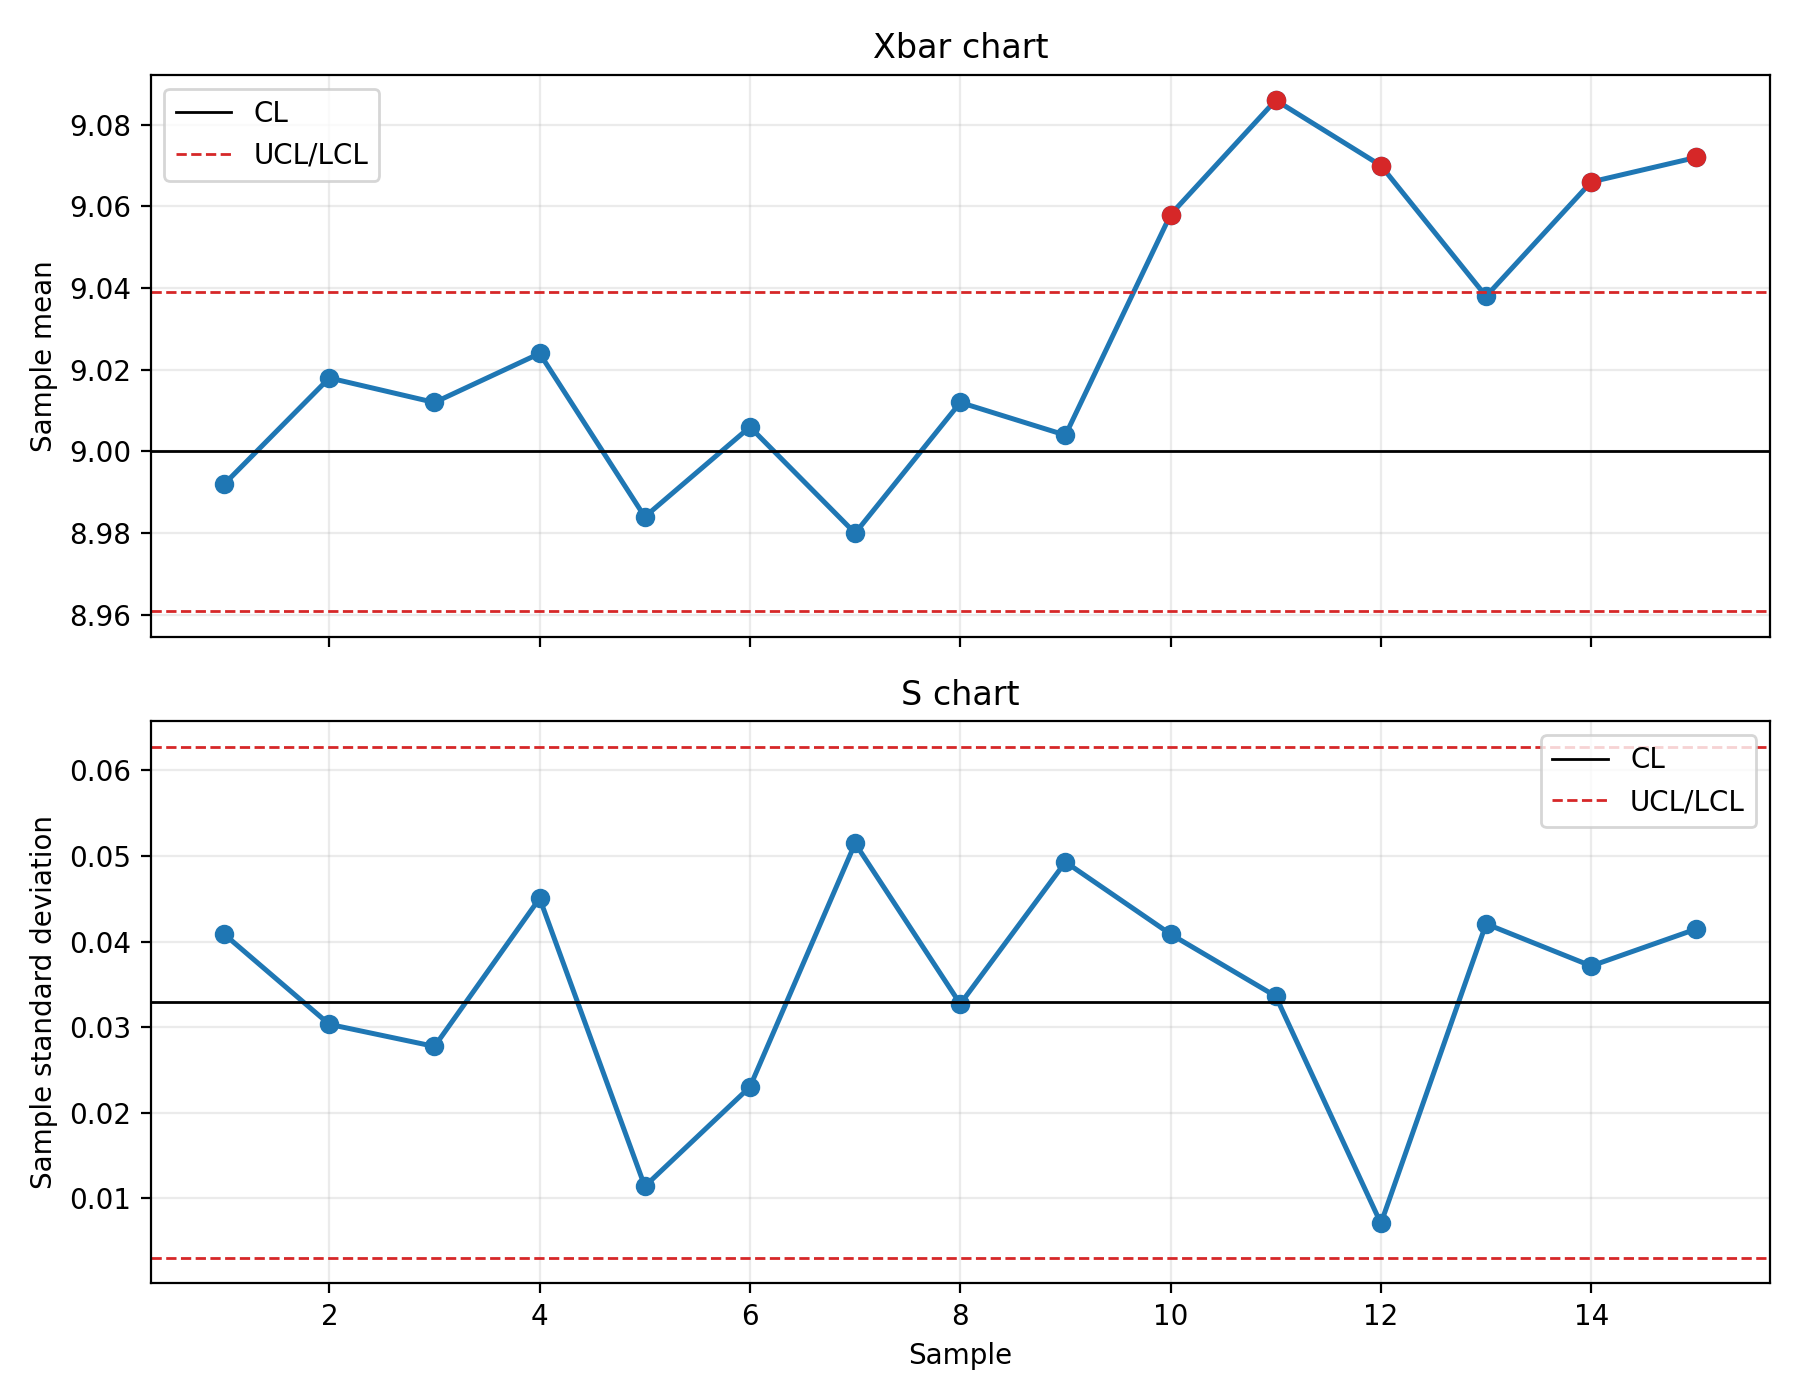
\includegraphics[width=0.92\textwidth]{control_charts_samples.png}
\caption{Διαγράμματα \(\bar X\) και \(S\) για τα 15 δείγματα.}
\label{fig:charts-v2}
\end{figure}

\subsubsection*{Ερμηνεία}

Τα δείγματα 10, 11, 12, 14 και 15 βγάζουν σήμα στο διάγραμμα \(\bar X\).
Δηλαδή πέντε ξεχωριστά σημεία πέφτουν πάνω από το \(UCL_{\bar X}=9{,}0391\).

Κανένα δείγμα δεν βγάζει σήμα στο διάγραμμα \(S\). Όλες οι δειγματικές
τυπικές αποκλίσεις είναι εντός \([0{,}003,\,0{,}063]\).

\begin{intuition}
Αυτός ο συνδυασμός είναι πολύ διαφωτιστικός. Αν η μεταβλητότητα είχε αυξηθεί,
περιμέναμε να βγουν τιμές στο \(S\). Δεν συμβαίνει αυτό. Αν αντίθετα είχε
γίνει μετατόπιση της μέσης τιμής προς τα πάνω, περιμέναμε σήματα στο
\(\bar X\) από κάποια στιγμή και μετά. Αυτό ακριβώς συμβαίνει: από το
δείγμα 10 και έπειτα, οι μέσες τιμές περνάνε επανειλημμένα πάνω από το
άνω όριο.
\end{intuition}

\subsubsection*{Συμπέρασμα}

\begin{center}
\fbox{\begin{minipage}{0.88\textwidth}
\centering
Η διαδικασία \emph{δεν} ήταν σε στατιστικό έλεγχο κατά τη διάρκεια των 15
δειγμάτων. Συγκεκριμένα, από το 10ο δείγμα και έπειτα εμφανίζεται ένδειξη
μετατόπισης της μέσης τάσης προς τα πάνω. Η μεταβλητότητα δεν φαίνεται να
έχει αλλάξει.
\end{minipage}}
\end{center}

\newpage

%=============================================================================
\section{Τελική σύνοψη}
%=============================================================================

Για να έχουμε όλα σε μία εικόνα, παρουσιάζουμε εδώ όλα τα αποτελέσματα της
εργασίας μαζί.

\subsection*{Μέρος Α: Δειγματοληψία αποδοχής}

\textbf{A1 -- απλό σχήμα:}
\[
    \boxed{(n,c)=(145,3)},\quad \Pa(p_1)=0{,}98470,\ \Pa(p_2)=0{,}09993,\ \AOQL=0{,}01016.
\]

\textbf{A2 -- διπλό σχήμα:}
\[
    \boxed{(n_1,n_2,c_1,c_2)=(75,75,0,3)},\quad \Pa(p_1)=0{,}98381,\ \ASN(p_1)=103{,}9.
\]

\textbf{A3:} Οι δύο OC είναι σχεδόν ταυτόσημες, καθώς και τα δύο σχήματα
καλύπτουν τις απαιτήσεις στα \(p_1\) και \(p_2\). Το διπλό σχήμα ελέγχει
λιγότερες μονάδες κατά μέσο όρο όταν η ποιότητα είναι καλή. Όταν η ποιότητα
είναι κακή, σχεδόν όλη η παρτίδα ελέγχεται και στα δύο σχήματα.

\textbf{A4 -- οικονομικά βέλτιστο απλό σχήμα με \(c\le 1\):}
\[
    \boxed{(n,c)=(189,1)},\quad E[C]=3.522{,}36 \text{ €/παρτίδα}.
\]

Το σχήμα του Α1 κοστίζει \(3.912{,}03\) €/παρτίδα, δηλαδή \(389{,}67\) €
περισσότερα ή περίπου 11\% πιο πολύ.

\subsection*{Μέρος Β: Διαγράμματα ελέγχου}

\textbf{B1 -- όρια:}
\[
    \bar X:\ [8{,}960869,\,9{,}039131],\quad
    S:\ [0{,}003043,\,0{,}062756].
\]

\textbf{B2 -- συνολική πιθανότητα ψευδούς συναγερμού:}
\[
    \boxed{\alpha_{\text{ολ}}=0{,}024364}.
\]

\textbf{B3 -- ισχύς του \(\bar X\) για μετατόπιση \(0{,}06\):}
\[
    \boxed{\text{χωρίς αύξηση σ: } 0{,}908777,\quad \text{με αύξηση σ: } 0{,}866727}.
\]

\textbf{B4 -- ισχύς του \(S\) για αύξηση σ κατά 20\%:}
\[
    \boxed{0{,}062919}.
\]

\textbf{B5 -- κόστος κακής ποιότητας μέχρι ανίχνευση:}
\[
    \boxed{159{,}56 \text{ € για τυχαία στιγμή μεταβολής}}.
\]

\textbf{B6 -- κατάσταση της διαδικασίας:} εκτός στατιστικού ελέγχου.
Πέντε δείγματα ξεπερνούν το \(UCL_{\bar X}\), κανένα δεν παραβιάζει το
διάγραμμα \(S\). Συμπεραίνουμε μετατόπιση της μέσης τάσης προς τα πάνω.

\subsection*{Παιδαγωγικό συμπέρασμα}

Η εργασία συνδυάζει δύο πολύ διαφορετικές οικογένειες προβλημάτων: αποδοχή
παρτίδων (offline) και παρακολούθηση παραγωγής (online). Σε κάθε περίπτωση
χρησιμοποιήσαμε λίγες αλλά κρίσιμες έννοιες: μια κατανομή (διωνυμική στο
Α, κανονική και \(\chi^2\) στο Β), δύο είδη σφαλμάτων (παραγωγού και πελάτη
στο Α, τύπου Ι και τύπου ΙΙ στο Β) και ένα οικονομικό κριτήριο (κόστος
ελέγχου και κόστος ελαττωματικών).

Όλη η εργασία απαντά στην ίδια κεντρική ερώτηση με δύο διαφορετικούς
τρόπους: ``πόσο πληροφορία αρκεί για να πάρω σωστή απόφαση, χωρίς να
σπαταλώ ούτε χρόνο ούτε χρήμα;''.

\end{document}
